% nastavení pro výpisy kódu
\renewcommand*\lstlistingname{Výpis}
\setlength{\parskip}{3pt plus 1pt minus 1pt}
\lstset
{
framexleftmargin=5mm,
frame=shadowbox,
rulesepcolor=\color{blue},
captionpos=b,
basicstyle=\footnotesize\ttfamily,
keywordstyle=\color{blue},
commentstyle=\color{OliveGreen},
stringstyle=\color{Maroon},
numbers=left,
numberstyle=\scriptsize,
stepnumber=2,
numbersep=5pt,
breaklines=true,
tabsize=2,
showstringspaces=false,
emph={double,bool,int,unsigned,char,true,false,void,get,set},
emphstyle=\color{blue},
emphstyle=\color{red},
emph={[2]\#using,\#define,\#ifdef,\#endif},
emphstyle={[2]\color{blue}},
frame=shadowbox
}
\newfloat{mylisting}{tbphH}{lopbl}[chapter]
\floatname{mylisting}{Výpis}
\newcommand{\cppc}[1]{\lstinline[language=C++]$#1$}

%\newsubfloat{mylisting}
%\newcommand{\listofmylistings}{\listof{mylisting}{List of Listings}}
% if you use the hyperref package
%\providecommand*\theHmylisting{\themylisting}
%=========================================================================
\chapter{Úvod}
V~moderních operačních systémech určených pro desktop (pracovní stanice, notebooky, etc.) se~oproti předchozím verzím změnilo mnohé. Jednou takovou změnou je~změna bezpečnostní politiky.

Bezpečnostní politiky zahrnují požadavky na operační systém a~to jak z~pohledu napadení systámu z~vnějšku, tak i~z~pohledu zabezpečení systému před lokálním uživatelem. Tato práce se~zabýva predevším bezpečnostními politikami pro lokální uzivatele. To zahrnuje jednak možnosti omezení chování uživatelů ve firemní síti, ale také domáci použití známe jako rodičovský režim.
V~případě firemního počítače se~může jednat například o~uzamčení jedné konkrétní konfigurace, aby ji zaměstnanci nemohli měnit. U~rodičovského módu se~může jednat o~omezení přístupu k~počítači na určitý čas, nebo omezení přístupu k~některým webovým serverům. Práce se~bude zabývat příbuzným tématem: integrací dvou rozhraní určených právě pro takovéto využití a~opravou grafického nástroje pro nastavení jednoho z~nich.

%%%%%

MS Windows postupně získal mnohem lepší zabezpečení ve verzích NT, kdy došlo k~přechodu na nové jádro, a~Vista, kde se~poprvé objevila možnost jednoduše povolit obyčejnému uživateli přístup k~nastavení systému pomocí UAC\footnote{User Access Control}. Zamezilo se~tak nutnosti \uv{být administrátorem}, což bylo do té doby výchozí nastavení po instalaci. Ve výsledku má uživatel povoleny akce, ke kterým by jinak přístup neměl.

Unixové a~unixu podobné systémy se~vyvíjely směrem opačným. Od práv pevně svázaných uživatelským účtem a~skupinou, k~mnohem volnějšímu pojetí. Za zmínku stojí například program sudo, který umožňuje uživateli spouštět programy s~jinými právy než jsou jeho vlastní (převážně superuživatelská práva) případně program su, který je~ještě staršího data. Novinkou je PolicyKit, který alespoň z~pohledu uživatele plní podobnou úlohu jako UAC na OS Windows. Aplikace využívající PolicyKit nemusejí mít pro změnu systémového nastavení jako je~třeba datum a~čas superuživatelská práva.

%%%% KDE

Původně byl všechen software KDE součástí jedné velké kolekce základních utilit pod názvem \uv{K~Desktop Environment}. Protože byly všechny programy a~knihovny součástí této jedné kolekce, stačilo ji vydávat pod jednotným názvem synchronizovaně. Jak tým KDE a~počet aplikací rostl, mnoho z~těchto programů začalo využívat své vlastní vývojové cykly a~oddělily se~od~původní kolekce.

KDE Software Compilation (dále KDE SC) je~množina knihoven a~programů vytvářených komunitou KDE, které stále používají původní synchronizovaný vývojový cyklus a~vytvářejí tak základ pro uživatelsky přívětivé grafické prostředí dostupné hlavně pro operační systém Linux, ale pracuje se~i~na verzích pro Windows a~Mac OSX.

KDE SC sestává z~knihoven KDE-Libs, které tvoří podklad pro všechny programy KDE a~mnoha balíků softwaru. KDEBase je~balík základních programů KDE a~obsahuje mimo jiné i~plochu Plasma a~prohlížeč souborového systému Dolphin (má podobný účel jako program Explorer ve Windows). Součástí KDE je~mnoho dalších balíků softwaru.

Prostředí KDE (po přeznačení KDE Software Compilation) je~možné provozovat na více operačních systémech. Aplikace by tak musely používat řešení jako je~UAC nebo PolicyKit, což by omezilo jejich přenositelnost. Tyto řešení tedy bylo potřeba nějak obalit. Za tímto účelem vzniklo rozhraní KAuth.\cite{whatiskde}

%%%% 

V~rámci KDE bylo možné již dříve měnit práva uživatelů -- skrývat položky menu, zamezit použití terminálu a~podobně. K~tomu slouží Kiosk, což je~framework postavený nad konfiguračním systémem KDE KConfig.

Práce se~z~velké části zabývá knihovnami v~balíku KDE-Libs a~rozhraními KAuthorized a~KAuth. Obě rozhraní slouží k~autorizaci akcí, které jsou v~rámci určité aplikace proveditelné uživatelem. Administrátor může použitím těchto rozhraní takovéto akce povolit nebo zakázat. Kiosk je~starší, postavený nad konfiguračním systémem KConfig a~má některá další specifika jako jsou zdroje dat nebo povolování přístupu~k~adresám URL. Zdroji dat rozumíme určitý typ souborů používaný v~aplikacích KDE. Například omezením pozadí na plochu, které se~řadí mezi zdroje dat (alespoň teoreticky) zamezíme tomu, aby uživatel mohl měnit pozadí plochy na jiné, než instalované v~systému. KAuth je~novějšího data a~je narozdíl od~Kiosku schopen také tyto akce provádět spouštěním pomocných programů s~jinými právy, než má jeho uživatel.

Společně s~nutnými základy bezpečnosti v~systému linux jsou tyto technologie a~způsob jakým budou v~práci využity blíže popsány ve druhé kapitole. Hlavním cílem práce je~integrovat KAuth do KAuthorized, aby mohl být používán pro ukládání povolení akcí a~přístupu ke zdrojům dat. Třetí kapitola integraci popisuje a~dále se~zabývá implementací nástroje pro migraci dat a~také pojednává o~testování systému jako celku. Další částí práce je~dokončení portu (přenesení) konfiguračního nástroje KioskTool z~prostředí KDE~3 do prostředí KDE~SC~4. Tímto se~zabývá kapitola čtvrtá. Pátá kapitola práci uzavírá a~navrhuje další možný postup.

\chapter{Použité technologie}
Tato kapitola se~zabývá popisem technologií použitých dále. Jedná se~zejména o~nástroje pro řízení přístupu \emph{subjektů} k~\emph{prostředkům} systému v~rámci uživatelského prostoru systému Linux. Subjektem mohou být například procesy, uživatelé nebo skupiny uživatelů. Prostředky pak mohou být soubory a~adresáře, zařízení (speciální typ souborů), čísla TCP a~UDP portů, nebo zmíněné akce autorizačních rozhraní KAuthorized a~KAuth.

Uživatelé se~do systému přihlašují, přičemž dochází k~ověření jejich identity, autentizaci. V~systému Linux lze řešit přihlašování pomocí mechanismu PAM\footnote{Pluggable Authentication Modules}. Ten umožňuje psát programy vyžadující autentizaci nazávisle na způsobu jakým je~jí dosaženo. Nezáleží pak, jestli se~uživatel přihlašuje heslem nebo například otiskem prstu. Další způsoby autentizace je~možné do systému doplnit pomocí zásuvných modulů. Podrobnější popis lze nalézt například v~článku, který vyšel na Root.cz\cite{rootpam}. Pokud je~to vyžadováno, KAuth využívá mechanismu PAM k~ověření totožnosti uživatele.

První část kapitoly se~zabývá přístupem subjektů k~souborům a~procesům. Je zde čerpáno z~dokumentu \cite{secureProg}, který je~vhodný pro hlubší studium problematiky a~knihy~\cite{OSP}, která je~obecněším úvodem. Část pojednávající o~Kiosku čerpá z~úvodu do Kiosku \cite{Kioskintro} a~zdrojového kódu kdelibs \cite{codeKdeLibs}. Část o~KAuth čerpá z~\cite{codeKAuth,KAuthusage}, v~části o~PolicyKitu je~čerpáno z~\cite{manpolkit_overview, manpolkit1, manpklocalauth}. Dříve než se~pustíme do samotného popisu technologií by bylo dobré prostudovat přílohu~\ref{pojmySeznam}.

\section{Souborový systém a~řízení přístupu k~souborům}
Unixu podobné operační systémy mají tzv. virtuální systém souborů, kde jsou všechny soubory na všech připojených souborových systémech umístěny v~jedné hierarchii. Tato hierarchie souborů a~adresářů má jeden kořenový adresář \uv{/}. Adresáře obsahují soubory a~platí, že adresář je~speciálním typem souboru (existují také další speciální soubory pro zařízení). Adresáře dále obsahují dvě speciální položky: \uv{..} odkazující na adresář o~úroveň výše a~\uv{.} odkazující na adresář samotný (identita).

V~hierarchii mohou být dále symbolické a~pevné odkazy. Symbolické odkazy mohou odkazovat jak na~soubory, tak na~adresáře. Při smazání odkazovaného souboru nebo adresáře symbolický odkaz zůstáva. Pevné odkazy pak mohou být pouze na soubory. Takto odkazovaný soubor je~smazán společně s~posledním pevným odkazem na~něj.

Ke každému souboru a~adresáři jsou přiřazena metadata, která popisují jejich další vlastnosti. Z~hlediska řízení přístupu je~podstatný uživatel a~skupina vlastnící soubor, práva pro čtení (r), zápis (w) a~spuštění (x) uživatelem, skupinou a~ostatními subjekty a~tzv. setuid a~setgid bity. U~obyčejných souborů označuje právo pro spuštění to, že je~to spustitelný program nebo skript. U~adresářů spustitelnost označuje fakt, že je~možné vypsat jejich obsah.\cite{secureProg, OSP}

Setuid bit určuje, že spuštěný program má běžet pod účtem vlastníka souboru. Setgid znamená to stejné pro skupiny. Bez nastavených setuid a~setgid bitů je~program spuštěn pod účtem uživatele, který jej spouští.\cite{secureProg}

%\section{Procesy a přístup k jejich prostředkům}
%TODO: Něco o tom, jak UID a GID funguji u procesu, jaky to ma vliv na pristup uzivatelum k pameti procesu, debugging a podobne.

\section{Kiosk}
Z~pohledu administrátora Kiosk nabízí možnost upravit si KDE pro své vlastní účely. Například schovat některé položky v~grafickém rozhraní aplikací, znemožnit uživatelům měnit nastavení a~data aplikací, zamezit spuštění terminálu nebo zcela zamknout nastavení všech aplikací. Z~pohledu programátora je~to jednoduché rozhraní umožňující autorizaci akcí, zdrojů dat pro aplikace a~přístupu k~adresám URL.

Kiosk je~vlastně framework, který kombinuje určité vlastnosti konfiguračního systému KConfig, jeho způsob načítání konfigurace z~tzv. Kiosk profilů, rozhraní KAuthorized a~specifikace, jakým způsobem jsou autorizace akcí uloženy v~KConfigu. Nelze přesně určit jedno konkrétní místo ve zdrojovém kódu KDE, kde by bylo popsáno jakým způsobem funguje, ale podrobným zkoumáním lze vysledovat, jak je~docíleno výsledného efektu.
%Obrázek: architektura Kiosk, Kconfig

\subsection*{KConfig}
Kconfig je~v~Kioksu použit pro uložení dat. Konfigurace je~uložena v~souborech podobných .INI souborům se~kterými se~dá jednoduše pracovat. Na rozdíl od~klasických INI souborů jsou však rozšířeny o~některé další vlastnosti.\cite{wikiINIfiles}
\begin{mylisting}
\caption{Ukázka konfiguračního souboru KConfig}
\label{kconf_exmpl}
\begin{lstlisting}[language=]
[$i]
[Colors]
CurrentPalette[$i]=Forty Colors

[ColumnMode]
FontWeight=50
PreviewSize=176

[DetailsMode]
FontWeight=50

[General][$i]
AutoExpandFolders=true
\end{lstlisting}
\end{mylisting}

Na výpisu \ref{kconf_exmpl} vidět, jak je~soubor členěn. Obsahuje skupiny a~záznamy typu klíč-hodnota. Soubory se~během načítání konfigurace slučují do jednoho konfiguračního objektu (třída KConfig), podle pořadí ve kterém jsou zpracovány. Jednotlivé skupiny z~načítaných souborů se~slučují do objektů typu KConfigGroup. Ty lze získat od~KConfig objektu podle jejich názvu. Pro pořadí zpracování konfiguračních souborů obecně platí, že globální systémová konfigurace je~zpracována jako první.

Celé soubory, skupiny jako je~\cppc{General} a~jednotlivé záznamy jako je~např. \linebreak\cppc{AutoExpandFolders} je~možné nastavit jako nezměnitelné (immutable) pomocí přidání značky \cppc{[\$i]}. Jakmile je~jednou nastavena na skupinu, soubor nebo hodnotu nezměnitelnost, jsou další objekty stejného typu při načítání ignorovány. V~uvedeném příkladu \ref{kconf_exmpl} je~nastavena nezměnitelnost pro klíč \cppc{CurrentPalette}, skupinu \cppc{General} a~celý soubor (první řádek). Máme-li tedy například nastavení programu Akregator (čtečka RSS) z~příkladu \ref{kconf_exmpl} umístěno v~některém adresáři s~globálním nastavením, budou položky, které jsou ve výsledku nezměnitelné uživatelům vnuceny. Uživatel je~pak sice stále může měnit ve vlastních konfiguračních souborech ve svém domovském adresáři, ale nezměnitelnost se~postará o~to, že budou takovéto změny ignorovány. Naopak, když nejsou položky v~globálním konfiguračním souboru nastaveny jako nezměnitelné, znamená to, že jsou chápány jako výchozí nastavení. Uživatel je~může měnit.

Je zřejmé, že řešení s~pouze jedním umístěním pro globální konfiguraci není ideální. Konfigurace se~pak totiž vztahuje na všechny uživatele systému. Kiosk proto zavádí tzv. Kiosk profily. Ty jsou vlastněny administrátorem (root) a~jsou nastaveny jako čitelné pro ostatní uživatele a~skupiny, kterým jsou přiřazeny. Dále je~popsáno načítání Kiosk profilů podrobněji.

\subsection*{Načítání konfigurace během spuštění aplikace}
Každá KDE aplikace má několik částí, obsažených ve jmenném prostoru \cppc{KGlobal}. Diagram~\ref{fig:kglobal} ukazuje, jak je~jmenný prostor \cppc{KGlobal} členěn. Obaluje přístup k~dalším komponentám a~sdíleným zdrojům v~rámci aplikace. \cppc{KComponentData} obsahuje informace relevantní pro jednu komponentu aplikace. Platí, že aplikace může mít jednu hlavní komponentu. \cppc{KAboutData} je~soubor základních informací o~programu. V~případě hlavní komponenty jsou tyto informace použity také pro dialog \uv{O~Aplikaci} (About). \cppc{KAboutData} určuje název komponenty a~ten se~použije pro načítání konfigurace a~pro výběr složky s~daty aplikace. Aplikace může mít více než jednu komponentu. \cppc{KSharedConfig} obsahuje sloučenou konfiguraci efektivní pro program a~zajišťuje, že konfigurace je~sdílena mezi komponentami. Šetří se~tak pamětí a~časem nutným k~načtení konfigurace. \cppc{KStandardDirs} slouží k~určení, které složky budou použity jako zdroj dat a~konfigurace pro aplikaci.

\begin{figure}[h]
    \centering
    \begin{verbatim}
            KGlobal ──┬── KComponentData ──┬── KAboutData
                      │                    ├── KStandardDirs
                      │                    └── KSharedConfig
                      ├── Locale
                      ├── nadpis okna
                      └── etc.\end{verbatim}
    \caption{Struktura KGlobal}
    \label{fig:kglobal}
\end{figure}

Právě \cppc{KStandardDirs} a~\cppc{KSharedConfig} jsou relevantní pro popis načítání konfigurace. Během inicializace komponenty se~nejdříve načítá obecná konfigurace. Ta obsahuje nastavení pro celé KDE a~zmíněnou aplikaci, ovšem bez začleněných Kiosk profilů. Potom je~volána metoda \cppc{KStandardDirs::addCustomized}, která vyhledá Kiosk profily platné pro uživatele a~zařadí je~mezi zdroje konfigurace s~prioritou. Soubor s~jejich seznamem je~odkazován z~\uv{/etc/kde4rc}.

Platí, že pokud má uživatel přiřazen svůj vlastní Kiosk profil, nezpracovávají se~dále Kiosk profily pro skupiny v~nichž je~členem. V~opačném případě, kdy uživatel nemá vlastní profil, přidají se~s~prioritou do cest v~KStandardDirs všechny aplikovatelné skupinové profily. Pokud se~počet cest s~konfigurací změnil, je~po návratu z~\cppc{addCustomized} konfigurace znovu načtena. Uživatelům, kteří nemají přiřazen žádný profil, je~přiřazen automaticky profil s~názvem \uv{default}. Opět platí, že jeho efekt je~zrušen jakýmkoliv přiřazeným skupinovým nebo uživatelským profilem, podobně jako uživatelské profily ruší efekt skupinových.

\subsection*{Rozhraní KAuthorized}
KAuthorized je~rozhraní postavené nad konfiguračním systémem KConfig a~využívá většiny jeho vlastností. Poskytuje knihovnám a~aplikacím KDE možnost autorizace obecných akcí, KAction akcí, konfiguračních modulů KControl, a~přistupů k~URL adresám. Chybí zde ovšem omezení přístupu ke zdrojům dat a~konfigurace.

Akce KAction (třída \cppc{KAction} odvozená od~\cppc{QAction} z~knihovny Qt) a~obecné akce jsou v~rámci KDE činnosti, které může uživatel vykonat v~aplikaci. Tyto akce mají název a~ten je~v~Kiosku použit pro jejich autorizaci. Jsou často asociovány s~nějakým ovládacím prvkem grafického rozhraní aplikace.

Restrikce akcí jsou nastavovány v~konfiguračních souborech ve skupině \linebreak\cppc{KDE Action Restrictions}. Zpravidla se~jich používá ke schování nebo vypnutí s~nimi provázaných prvků rozhraní. Akce může být například otevření menu s~nápovědou, změna pozadí na ploše nebo vypnutí počítače z~menu KDE. Pokud je~taková akce zakázána pomocí Kiosku, prvky uživatelského rozhraní se~nezobrazí (případně nevytvoří během inicializace aplikace).

Rozdíl mezi obecnou akcí a~akcí KAction je~v~rámci \cppc{KAuthorized} mizivý a~funkce \linebreak\cppc{AuthorizeKAction} je~obal nad \cppc{authorize}, který před název akce přidá prefix \uv{action/}. Příslušná funkce pak použije globální \cppc{KConfig} objekt aplikace k~ověření, zda má uživatel tuto akci zakázánu (ve výchozím stavu jsou všechny povoleny).

Omezení přístupu ke zdrojům je~nastavováno ve skupině \cppc{KDE Resource Restrictions} a~je umístěno do globálního konfiguračního souboru jako je~\cppc{kdeglobals}. Omezením zdrojů lze docílit toho, že aplikace \uv{neuvidí} zdroje umístěné v~uživatelově domovské složce. Lze tak zamezit například tomu, aby si uživatel aplikace rozšiřoval. I~když je~tato část Kiosku velmi podobná ostatním autorizačním funkcím v~\cppc{KAuthorized}, není do něj přímo začleněna. Důvodem je, že je~úzce provázána s~třídou \cppc{KStandardDirs}, která tyto omezení zpracovává a~používá pro vytvoření seznamů složek se~zdroji. Seznam těchto omezení je~potřeba znát ještě před tím, než je~zcela načtena konfigurace z~jednoho prostého důvodu -- je~možné omezit i~zdroj pro konfiguraci. Zde bude nutné poupravit způsob načítání konfigurace tak, aby bylo možné umístit omezení na zdroje dat i~do Kiosk profilů.

%ref: http://techbase.kde.org/KDE_System_Administration/Kiosk/Introduction#KDE_URL_Restrictions
Omezení přístupu k~URL je~nastavováno ve skupině \cppc{KDE URL Restrictions}. Tyto omezení jsou určeny pro zamítnutí přístupu k~některým adresám URL.

Dalším typem omezení jsou tzv. \cppc{KDE Control Module Restrictions}, které se~používají ke skrytí nebo zamezení otevření konfiguračních dialogů. KDE používá třídu \cppc{KCModule} jako základ pro všechny moduly použité v~aplikacích \uv{Nastavení Systému}, \cppc{kcmshell} a~případně v~jiných aplikacích, které používají tyto moduly pro úpravu svého nastavení. Omezení se~vztahují k~názvům těchto modulů. Pokud budou moduly přejmenovány, přestanou omezení fungovat.

\section{KAuth}
KAuth je~nové rozhraní pro autorizaci v~KDE. Je postaveno na již existujících rozhraních v~operačních systémech. V~OS na bázi Linuxu je~to zpravidla PolicyKit, v~OSX pak framework Authorization Services. Podporu pro nová rozhraní je~možné přidat připsáním nových zásuvných modulů.

Pomocí KAuthu je~možné autorizovat akce uživatele a~také je~provádět. Akce jsou prováděny za použití pomocného programu, který je~spuštěn příslušným autorizačním rozhraním přítomným v~systému. Takovýto program se~nazývá KAuth pomocník (helper). Pomocník a~aplikace která ho využívá mohou do jisté míry komunikovat oběma směry a~je také možné sledovat průběh dlouho trvající akce uvnitř pomocníka. KAuth pomocník je~rozšířením PolicyKit pomocníka o~tyto zjednodušené komunikační funkce. Hlavní výhodou je, že za použití pomocníka lze provádět privilegované akce bez nutnosti být přihlášen pod administrátorským účtem nebo tohoto účtu používat ke spuštění aplikace jako celku.

Další službou KAuthu je~registrace pomocníků a~akcí v~jeho jednotlivých zásuvných modulech. Uživatel KAuthu tedy specifikuje, jaké akce a~pomocníky chce použít a~při kompilaci budou tyto specifikace převedeny do formy srozumitelné pro jeho zásuvné moduly.

Díky tomu jakým způsobem je~KAuth navržen, nepodporuje provádění změn v~seznamu platných akcí po kompilaci. Také neumožňuje měnit autorizované uživatele a~skupiny pro akce. To je~zcela přenecháno použitému autorizačnímu systému. Dále pak platí omezení na názvy KAuth akcí, které mohou obsahovat jen malá písmena anglické abecedy, číslice a~tečku jako oddělovač.

\subsection*{Formát specifikace akcí}
Formát specifikace akcí je~podobný jako formát konfiguračních souborů KConfig. Obsahuje skupiny a~záznamy klíč-hodnota v~těchto skupinách. Uvedený příklad .actions souboru \ref{fig:kauth_dotactions} byl použit k~vygenerování podobného souboru pro PolicyKit, který je~uveden dále ve výpisu \ref{fig:pkit_policy}.

\begin{mylisting}
\caption{Ukázka KAuth .actions souboru}
\label{fig:kauth_dotactions}
\begin{lstlisting}
[Domain]
Name=Date and Time Control Module
Icon=preferences-system-time

[org.kde.kcontrol.kcmclock.save]
Name=Save the date/time settings
Description=System policies prevent you from saving the date/time settings.
Policy=auth_admin
Persistence=session
\end{lstlisting}
\end{mylisting}

Soubor obsahuje skupinu Domain, která popisuje, ke které aplikaci patří a~jakou má mít ikonu. V~tomto případě se~jedná o~KControl modul pro nastavení data a~času. Textové položky mohou být lokalizovány (zde vynecháno).

Po skupině Domain následují definované akce. Platí, že název akce je~také názvem skupiny v~souboru. Název akce se~skládá ze dvou částí: jmenného prostoru a~názvu akce v~něm. Zde je~jmenným prostorem část \cppc{org.kde.kcontrol.kcmclock} a název akce je~\cppc{save}. Skupina dále obsahuje srozumitelný název (\cppc{Name}), popis (\cppc{Description}) a~výchozí chování při pokusu o~autorizaci.

Položka Policy určuje průběh autorizace. V~případě, že je~nastavena na hodnotu \cppc{yes}, je~autorizace okamžitá. \cppc{no} naopak znamená, že akce nemůže být autorizována. Pokud je~nastavena na \cppc{auth_self}, bude akce autorizována pokud se~uživatel přihlásí pod svou vlastní identitou. Konečně \cppc{auth_admin} znamená, že akce bude autorizována pokud se~uživatel přihlásí jako administrátor.

Poslední položkou skupiny je~\cppc{Persistence}. Ta je~nepovinná a~udává, na jak dlouho bude autorizace udělena. Možnostmi jsou \cppc{session}, kdy bude platit dokud se~neodhlásí a~\cppc{always}, kdy nebude omezena.

Specifikace akcí v~.actions souborech je~také dále omezená tím, že všechny názvy akcí v~jednom souboru musejí mít společný základ (jmenný prostor).

\subsection*{Rozhraní KAuth}
KAuth poskytuje jednoduché rozhraní pro práci s~akcemi. Jeho základem je~třída \cppc{KAuth::Action}, kterou lze využít pro autorizaci akcí a~spouštění KAuth pomocníku. Funguje jako rozhraní nad jednotlivými autorizačními systémy a~používá je~prostřednictvím zásuvných modulů založených na třídě \cppc{KAuth::AuthBackend}. Vztah mezi těmito třídami je~znázorněn na diagramu \ref{fig:KAuthDiag}. Akce přijímá jako parametr konstruktoru jméno. K~autorizaci pak slouží její jednotlivé metody. Diagram byl zjednodušen, celou dokumentaci k~rozhraní KAuth lze nalézt na stránkách KDE.\cite{KAuthusage, KAuthAPI}


\begin{figure}[h]
    \centering
    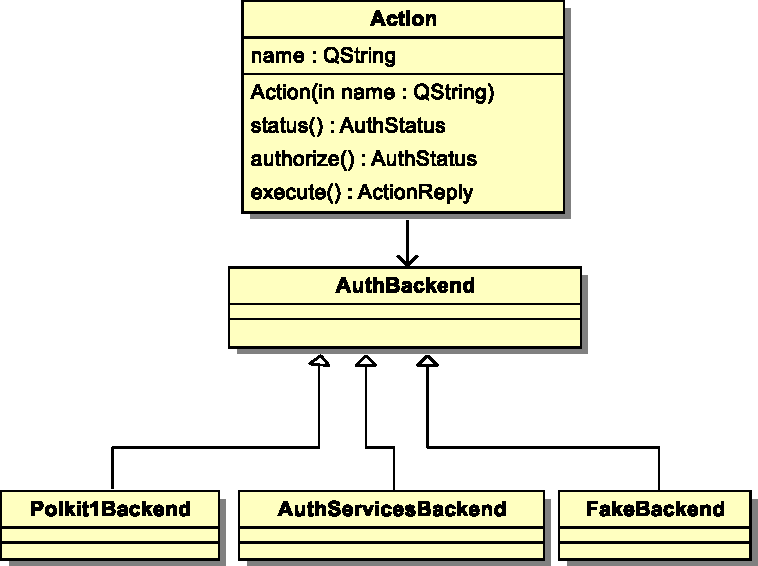
\includegraphics[width=6cm]{obrazky/KAuthAction.pdf}
    \caption{Vztah mezi KAuth::Action a~KAuth::AuthBackend}
    \label{fig:KAuthDiag}
\end{figure}

\section{PolicyKit}
\begin{figure}[h]
    \centering
    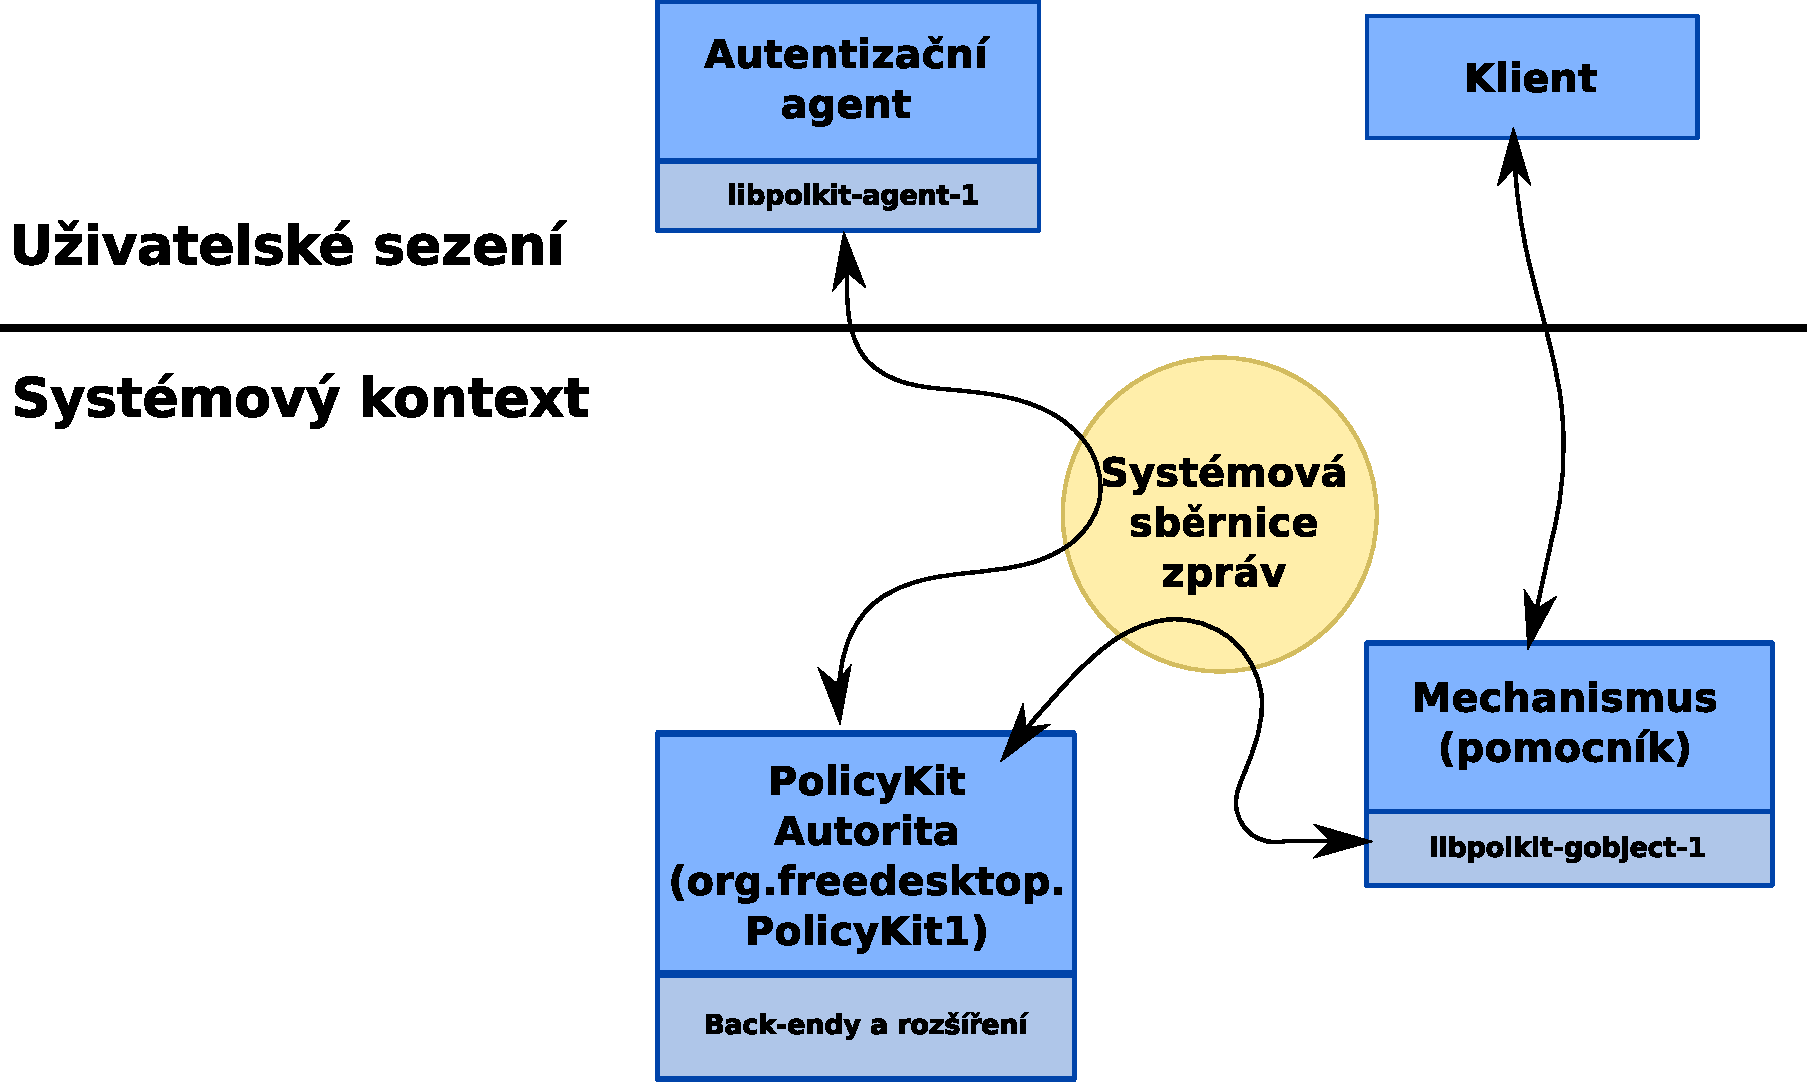
\includegraphics[width=12cm]{obrazky/polkit-architecture-vector-cz.pdf}
    \caption{Architektura systému PolicyKit, přeloženo z~\cite{manpolkit1}}
    \label{fig:polkit_arch}
\end{figure}

V~této sekci jsem čerpal z~manuálu \cite{manpolkit_overview}, převážně pak z~jeho částí \cite{manpolkit1} a~\cite{manpklocalauth}.

PolicyKit poskytuje autorizační rozhraní privilegovaným programům (mechanismy), které nabízejí služby neprivilegovaným programům (klienti) za použití IPC\footnote{Inter-process communication} mechanismu jako je~D-Bus. Pro ilustraci propojení jednotlivých částí dobře poslouží diagram \ref{fig:polkit_arch}. Mechanismus považuje požadavky od~klienta za nevěrohodné a~pro každý požadavek musí mechanismus zjistit, jestli je~autorizován nebo jestli má klientovi službu odepřít. Pomocí PolicyKit API může mechanismus tuto část přenechat důvěryhodné třetí straně: PolicyKit autoritě.\cite{manpolkit1}

Vedle funkce jako autorita umožňuje PolicyKit uživatelům také získat dočasnou autorizaci pomocí autentizace jakožto administrátor nebo vlastník sezení do kterého klientský program patří. To je~výhodné v~situaci, kfy je~nutné ověřit totožnost osoby používající klientský program.\cite{manpolkit1}

Tedy podobně jako KAuth, PolicyKit umožňuje autorizovat akce uživatelů a~pomocí tzv. mechanismů tyto akce provádět. Jádrem PolicyKitu je~několik základních komponent. První důležitou částí je~démon polkitd, který funguje jako centrální prvek PolicyKitu a implementuje část PolicyKit Authority, která se~stará o~čtení databáze možných akcí a~povolení nebo zamítnutí požadovaných akcí.

Další částí, implementovanou prostředími jako je~Gnome nebo KDE je~tzv. autentizační agent. To je~program, který například uživateli zobrazí okno pro zadání hesla, pokud je~potřeba ověřit jeho totožnost. Pro samotné ověření je~možné použít pomocný program běžící se~superuživatelskými právy (za pomocí setuid bitu) a~používající k~ověření systém jako je~PAM. Ten je~dobře popsán v~článku \cite{rootpam}. Autentizace ale nemusí být striktně vyžadována. Lze i~jen zobrazit obyčejné okno s~dotazem typu Ano/Ne.

Třetí komponentou je~\uv{mechanismus} nebo \uv{pomocník}. zde se~jedná o~službu pro vykonání privilegovaných akcí místo uživatele, který o~provedení akce žádá. Čtvrtou a~poslední komponentou je~klient. To je~program, který využívá služeb systému PolicyKit.


% http://lists.freedesktop.org/archives/polkit-devel/2009-July/000153.html

Průběh akcí v~systému pro volání funkce pomocníka může vypadat například takto:
\begin{itemize}
\item Uživatel se~přihlásí, je~nastartováno sezení KDE a~s~ním i~autentizační agent
\item Autentizační agent se~registruje u~PolicyKit autority
\item Uživatel spustí program, který využívá služeb PolicyKitu
\item Program zavolá funkci pomocníka přes systém D-Bus
\item DBUS démon nastartuje program pomocníka, pokud již neběží (pomocník musí být v~systému D-Bus registrován)
\item Spuštěný pomocník se~zeptá PolicyKit autority, jestli je~volaná akce autorizována
\item PolicyKit autorita zkontroluje, jestli je~již tato akce autorizována (autorizace může mít například platnost po délku celého sezení). Pokud není zatím autorizována, zjistí jakým způsobem se~má autorizace dosáhnout.
\item Pokud je~to nutné, zavolá PK autorita autentizačního agenta. Je možné ověřovat buď pouze identitu uživatele, kdy stačí, že se~přihlásí pod vlastním účtem, nebo je~možné vyžadovat přihlášení účtu se~superuživatelskými právy.
\item Uživatel se~přihlásí. Ve většině distribucí Linuxu za pomoci mechanismu PAM.
\item Agent oznámí autoritě jestli byla autentizace úspěšná.
\item Autorita vrací výsledek autorizace a~uloží si ho do vyrovnávací paměti po dobu její platnosti.
\item Pokud byl proces autorizace úspěšný, pomocník provede požadovanou akci.
\item V~tomto bodě může pomocník oznámit programu výsledek akce.
\end{itemize}

Toto samozřejmě není jediný možný průběh. Je například možné přistupovat k~PolicyKit autoritě z~klientského programu a~pouze požadovat autorizaci akcí bez použití pomocníka. Právě to bude přístup použitý v~další kapitole.

Nad PolicyKitem je~postavena knihovna polkit-qt, která poskytuje v~zásadě stejné funkce jako PolicyKit a~lépe je~integruje do prostředí knihoven Qt. Polkit-kde je~nadstavbou nad knihovnou polkit-qt, která implementuje autentizační agent pro prostředí KDE.

Zatím jediným způsobem uložení povolených akcí v~PolicyKitu je~tzv. lokální autorita (PolicyKit Local Authority). Je to výchozí implementace PolicyKit Autority a~využívá lokálně uložených textových souborů s~příponou .policy a~.pkla. Nejdříve příklad \ref{fig:pkit_policy} .policy souboru. Tyto soubory používají formát XML a~vymezují seznam známých akcí. Instalují se~do systému jako součást balíčků, jsou vlastněny administrátorem a~nejsou čitelné pro ostatní uživatele.

Značka \cppc{vendor} určuje k~čemu tento soubor akcí patří. V~tomto případě je~to KControl modul pro nastavení data a~času. Soubor má dále nastavenu ikonu a~samotný seznam akcí. Akce má popis (description), zprávu pro případ neúspěšné autorizace (message) a~výchozí nastavení autorizace. PolicyKit rozlišuje mezi tzv. aktivním a~pasivním sezením. Aktivní je~například normálně přihlášený uživatel s~vlastním X serverem. Pasivní může být sezení spuštěné dodatečně z~login terminálu (su - username). Normálně může být aktivní pouze jedno sezení (to s~kterým uživatel zrovna přímo pracuje). Dalším povoleným typem atributu je~tzv. anotace. Anotace umožňuje přidat k~akci další atributy. Soubor povoluje měnit nastavení času pouze uživateli s~aktivním sezením, který se~prokáže jako superuživatel.

\begin{mylisting}
\caption{Ukázka souboru s~definicí akce (.policy soubor), soubor byl generován KAuthem ze souboru \ref{fig:kauth_dotactions}}
\label{fig:pkit_policy}
\begin{lstlisting}[language=XML]
<?xml version="1.0" encoding="utf-8"?>
<!DOCTYPE policyconfig PUBLIC
"-//freedesktop//DTD PolicyKit Policy Configuration 1.0//EN"
"http://www.freedesktop.org/standards/PolicyKit/1.0/policyconfig.dtd">
<policyconfig>
<vendor>Date and Time Control Module</vendor>
<icon_name>preferences-system-time</icon_name>
   <action id="org.kde.kcontrol.kcmclock.save" >
      <description>Save the date/time settings</description>
      <message>System policies prevent you from saving the date/time settings.</message>
      <defaults>
         <allow_inactive>no</allow_inactive>
         <allow_active>auth_admin</allow_active>
      </defaults>
   </action>
</policyconfig>
\end{lstlisting}
\end{mylisting}

Takto vymezené akce je~dále možné pozměnit v~souborech .pkla. Efektivní seznam povolených akcí se~získá sloučením záznamů z~těchto souborů. Je tedy možné mít například jeden soubor s~nastavením instalovaný z~distribučního balíčku a~druhý s~vyšší prioritou vytvořený administrátorem. Stejně jako soubory se~specifikacemi akcí nejsou soubory Local Authority čitelné ostatními uživateli.

Local Authority pro ně zavádí poměrně propracovanou strukturu složek ve dvou umístěních (/var/lib/polkit-1/localauthority a~/etc/polkit-1/localauthority). Pořadí načítání je~určeno lexikografickým řazením složek a~souborů v~nich. Pokud je~stejně pojmenovaný soubor v~obou umístěních, nejdříve se~zpracuje ten ve /var/. Detaily a~příklad viz. \cite{manpklocalauth}.

\begin{mylisting}
\caption{Ukázka souboru s~nastavením PolicyKit Local Authority, Přeloženo z~\cite{manpklocalauth}}
\label{fig:pkit_pkla}
\begin{lstlisting}
[Povolene akce pro zamestnance]
Identity=unix-group:zamestnanci
Action=com.example.uzasnyprodukt.*
ResultAny=no
ResultInactive=no
ResultActive=yes

[Zakazy pro par cernych ovci]
Identity=unix-user:petr;unix-user:pavel
Action=com.example.uzasnyprodukt.*
ResultAny=no
ResultInactive=no
ResultActive=auth_admin
\end{lstlisting}
\end{mylisting}

Na výpisu \ref{fig:pkit_pkla} je~ukázka .pkla souboru. Uživatelé petr a~pavel jsou členy skupiny zamestnanci.

Záznamy se~v~rámci souboru zpracovávají tak jak jdou za sebou a~platí, že zpracování pokračuje i~po úspěšném porovnání uživatelského jména/skupiny s~těmi od~žadatele. Procházi se~tedy vždy všechny záznamy. Jako příklad si vezmu uživatele petr, který požádá o~autorizaci akce \cppc{com.example.uzasnyprodukt.uzasnaakce}. Zaměstnanci mají tuto akci obecně povolenu bez nutnosti se~přihlašovat v~první skupině souboru. Zpracování však pokračuje a~uživatel petr se~bude muset pro úspěšnou autorizaci akce přihlásit jako administrátor.

Rozdíl mezi položkami \cppc{ResultAny}, \cppc{ResultInactive} a~\cppc{ResultActive} se~nemusí zdát zjevný. \cppc{ResultActive} a~\cppc{ResultInactive} jsou výsledky akce pro aktivní a~neaktivní sezení, podobně jako značka \cppc{allow_active} a~\cppc{allow_inactive} v~.policy souborech. \cppc{ResultAny} pak určuje výsledek pro oba typy sezení. Alespoň jedna z~těchto položek musí být přítomna. Hodnota položky udává jakým způsobem bude uživatel žádající o~autorizaci akce autentizován.

\chapter{Integrace KAuth do KAuthorized}
\section{Analýza problému}
První praktickou částí projektu je~zjistit jak nejlépe integrovat systém KAuth do rozhraní KAuthorized. Díky celkové rozdílnosti KAuthu a~KAuthorized bude nejspíše potřeba určitých kompromisů.

Na jedné straně Kiosk, podporující profily přiřazené uživatelům a~skupinám a~změnu těchto profilů (stačí být administrátor a~upravovat profily standardními nástroji). Na druhé straně KAuth, primárně určený k~odstranění nutnosti spouštět programy pro systémovou konfiguraci s~grafickým uživatelským rozhraním jako administrátor.

\subsection*{Varianta s~přímou integrací}
První a~nejjednodušší varianta je~vytvořit statický .actions soubor (poté přeložený KAuthem) v~kombinaci s~integrací KAuth přímo do rozhraní KAuthorized. KAuth by tak konvertoval tento statický soubor do formy srozumitelné pro PolicyKit během sestavení KDE-Libs.

Problémem je~zde to, že neexistuje definitivní seznam možných restrikcí akcí a~zdrojů v~Kiosk profilech. Toto by šlo řešit tak, že každý program KDE by tyto své akce a~zdroje specifikoval v~.actions souboru k~tomu určeném a~zahrnul by jeho překlad do svého sestavení. To ovšem vylučuje jakoukoliv možnost stejné úrovně podpory pro aplikace, které by takto akce nespecifikovaly.

Druhým problémem je~neexistence možnosti nastavit autorizované akce pro uživatele a~skupiny pomocí KAuthu. Nejen že nejdou nastavit, KAuth navíc nemá ani žádné ponětí o~něčem, co by alespoň vzdáleně připomínalo způsob jakým se~aplikují Kiosk profily. V~případě použití PolicyKitu tyto vcelku základní funkce nemá ve formě knihovny žádná vrstva - PolicyKit, polkit-qt, polkit-kde ani KAuth. Musí se~přímo přistupovat ke konfiguračním souborům PolicyKitu.

Tato varianta vyžaduje implementaci nástroje pro překlad Kiosk profilů na nastavení KAuth/PolicyKit. Zde je~nutno přihlédout k~tomu, že názvy akcí v~KAuthu jsou daleko více omezené než ty v~Kiosku. Všechny akce v~jednom .actions souboru musejí mít společný jmenný prostor a~v~PolicyKitu soubor musí být podle tohoto jmenného prostoru pojmenován. Navíc mohou názvy obsahovat pouze malá písmena latinky, číslice a~tečku jako oddělovač. Názvy akcí a~zdrojů v~Kiosku tato omezení samozřejmě nemají a~často využívají jiné znaky jako je~například pomlčka, podtržítko nebo lomítko. Tyto znaky je~potřeba buď odstranit nebo nahradit. Vzniká tak reálná možnost kolize názvů.

\subsection*{Varianta s~KConfig objektem v~KAuth pomocníkovi}
Druhá možná varianta je~jednoduše se~vzdát mapování akcí mezi Kioskem a~KAuthem jedna ku jedné. Mělo by být možné umístit do KAuth pomocníka obsahujícího instanci KConfigu, která načte požadované Kiosk profily a~bude přes KAuth/D-Bus umožňovat dotazování se~na jednotlivé hodnoty v~nich. Bylo by také možné tyto hodnoty měnit. V~podstatě by to byl stále pouze KConfig, jen obalen v~pomocníkovi. I~toto řešení by však mělo problémy.

Nezíská se~tím vůbec výhoda z~pohledu bezpečnosti. Kiosk profily musejí stále zůstat čitelné pro všechny uživatele, jinak by se~při spuštění programů nemohly načíst a~části které nebudou takto integrovány v~pomocníkovi (vše s~výjimkou omezení akcí a~zdrojů) by tím byly zcela neefektivní. Odpadá tak výhoda KAuthu, kde jak seznam omezení, tak jaká omezení pro koho platí může být před uživateli skryt. Při použití PolicyKit Local Authority je~možné nastavit všechny soubory čitelné jenom superuživatelem (dokonce je~to výchozí stav).

KAuth pomocníci mají omezenou životnost. Pokud nejsou využíváni po dobu deseti vteřin, jsou ukončeni (viz. zdrojový kód KAuth \cite{codeKAuth}). Znamená to znovu načíst celý KConfig objekt. I~když je~toto načítání vysoce optimalizováno, stále je~vcelku zbytečné načítat celou konfiguraci dvakrát. Jednou v~programu, který by volal KAuthorized a~podruhé v~KAuth pomocníkovi. Sdílet zde jeden konfigurační objekt by bylo zbytečně komplikované, protože se~jedná o~dva procesy, navíc spuštěné s~jinými právy.

Jedna z~vlastností KAuthu, kterou by se~také nedalo využít jsou srozumitelné názvy akcí v~systému. Místo \cppc{org.kde.kiosk.action.help} a~mnoha dalších by byly v~systému jen akce pomocníka. V~tom případě se~ovšem nedá mluvit o~integraci KAuthu a~KAuthorized.

V~této variantě by nebylo potřeba implementovat nástroj pro překlad Kiosk profilů na nastavení KAuth/PolicyKit.

\subsection*{Další požadavky na řešení}
Použití KAuthu by nemělo být povinné a~mělo by být zachováno chování rozhraní \cppc{KAuthorized} pokud možno tak, aby se~z~pohledu aplikací nic nezměnilo. Zde je~problém to, že administrátor může, ale také nemusí nastavit v~systému \cppc{KConfig} kteroukoliv položku jako nezměnitelnou. Pokud bude kontrola oprávnění pomocí KAuthu před kontrolou pomocí KConfigu, je~nutné zaručit, že omezení známá v~KAuthu mohou být brána jako změnitelná, tak aby mohly být dále modifikována pomocí nastavení v~KConfigu. KAuth ani PolicyKit toto neumožňují. Musí se~také počítat s~tím, že KAuth nemusí být přítomen v~systému nebo že konvertor zatím nikdy nebyl spuštěn a~v~těchto případech použít normální nastavení Kiosk profilu přes \cppc{KConfig}.

\section{Návrh řešení}\label{mozres}
Rozhodl jsem se~implementovat první variantu. To znamená přímo integrovat KAuth do rozhraní KAuthorized. Samotná integrace bude vyžadovat mnoho malých změn v~KDE-Libs a~implementaci nástroje pro konverzi Kiosk profilů na nastavení lokálního systému pro autorizaci. Zde se~budu držet PolicyKitu a~operačního systému Linux.

Konvertor bude fungovat jako KAuth pomocník a~bude vytvořen samostatný program spustitelný uživatelem z~příkazové řádky, který bude tohoto pomocníka volat. Konverze z~Kiosk profilů bude jednosměrná, bude používat polkit-qt pro získání seznamu podporovaných omezení a~bude produkovat soubory .pkla, použitelné v~PolicyKit Local Authority. Konvertor by mělo být možné, až bude stabilní, integrovat do KAuthu nebo balíku policykit-kde. Konvertor nebude vyžadovat od~uživatele žádný vstup.

V~konvertoru je~nutné zohlednit to, že postup aplikace profilů v~Kiosku je~jiný než postup ověření autorizace v~PolicyKitu. Musí se~replikovat Kiosk a~jeho zvláštnosti, aby se~nezměnilo chování KAuthorized. Problém s~omezeními názvů akcí v~KAuth v~porovnání s~Kioskem je~nutné řešit buď záměnou znaků v~názvech akcí z~Kiosku, nebo překódování celých názvů do přijatelné a~v~KAuthu uložitelné podoby.

Integrace KAuth do KAuthorized je~sice otázka několika volání funkcí KAuth, ale autorizační funkce KAuthu na rozdíl od~systémů na kterých staví nevrací chybové kódy v~případě, že akce neexistuje. Toto bude potřeba do KAuthu doplnit.

Omezení na zdroje \cppc{KDE Resource Restrictions} si vyžádají změny ve třídě \cppc{KStandardDirs}. Bude potřeba doplnit schopnost načítat omezení zdrojů z~Kiosk profilů a~umístit do jmenného prostoru \cppc{KAuthorized} funkci, která bude vracet seznam typů zdrojů s~nastaveným omezením.

\section{Implementace}
\subsection*{Změna v~KAuth}
Implementace spočívá v~několika přesně cílených změnách v~kódu KDE-Libs. V~prvé řadě byla doplněna schopnost KAuthu vracet vedle informace o~úspěšnosti autorizace také zvláštní hodnotu pro případ, že akce není použitému systémem pro autorizaci známa. Ve výchozím stavu vypadá funkce pro získání autorizace jak je~znázorněno v~příloze \ref{kauth-oldmethod}. Hodnota \cppc{Unknown} je~vrácena v~případě, kdy dojde k~chybě během autorizace. Důvod chyby lze zjistit bližším dotazováním autorizačního rozhraní. Úprava metody pak je~v~příloze \ref{kauth-newmethod}.

\subsection*{Přesun vyhodnocení omezení na zdroje do KAuthorized}
Zjišťování seznamu omezení na zdroje je~umístěno v~metodě \cppc{addCustomized} třídy \cppc{KStandardDirs} a~tento seznam je~vytvářen před tím, než se~načtou Kiosk profily. Tato metoda přidává profily k~cestám pro načítání konfigurace a~třída \cppc{KComponentData}, která tuto metodu volá následně způsobí znovunačtení konfigurace. Z~takovéto načtené konfigurace již nejsou vytaženy seznamy omezení zdrojů.

Rozhodl jsem zjišťování seznamu omezených zdrojů přesunout do rozhraní \cppc{KAuthorized}, aby byly změny nutné pro integraci KAuthu pokud možno pouze na jednom místě.

Dále jsem se~rozhodl, že oddělím zpracování tohoto seznamu od~metody \cppc{addCustomized()}. Dá se~tak spustit z~třídy \cppc{KComponentData} poté, co \cppc{KStandardDirs} přidá Kiosk profily mezi konfiguraci. Tím se~docílí toho, že je~možné uložit omezení zdrojů stejným způsobem jako omezení na akce.

Implementoval jsem tedy funkci \cppc{restrictResourceTypes} pro získání seznamu Kioskem neomezených zdrojů ve formě objektu \cppc{QStringList} a~umístil ji do rozhraní KAuthorized. Dále jsem přesunul vyhodnocení těchto omezení do nové metody \linebreak\cppc{evaluateRestrictedResources()} v~\cppc{KStandarDirs}, která je~volána po znovu-načtení konfigurace po přidání profilů. Bylo nutné také změnit konstruktor privátního objektu v~KAuthorized, aby neblokoval zpracování profilů. Původně nebyl navržen na to, aby byl použit tak brzo během spouštění programů.

\subsection*{Specifikace akcí a~zdrojů}
Ke specifikaci akcí v~systému KAuth jsou využity statické .actions soubory. Jako základní jmenný prostor jsem se~rozhodl použít \cppc{org.kde.kiosk}. Pro akce jsem se~rozhodl pro \cppc{org.kde.kiosk.action} a~pro zdroje \cppc{org.kde.kiosk.resource}.

Názvy akcí a~zdrojů nemohou obsahovat jiné znaky než malá písmena a~číslice. Je tedy nutné přeložit jejich skutečné názvy do formy, kterou je~KAuth schopen použít. Z~akce \cppc{action/help} se~tak stane \cppc{actionhelp}, společně se~jmenným prostorem pak \linebreak\cppc{org.kde.kiosk.action.actionhelp}. Kdyby však exitovala jiná akce s~názvem \cppc{action\_help}, došlo by ke kolizi.

\subsection*{Implementace konvertoru}
Konvertor se~skládá ze dvou částí. Hlavní částí je~pomocník, postavený na knihovně KAuth. Ten implementuje veškeré funkce celku (ve zdrojovém kódu je~to kdelibs/kdecore/auth/kioskpklahelper.cpp). Druhou částí je~jednoduchý terminálový program, který není až na~spuštění pomocníka přes KAuth příliš zajímavý (ve zdrojových kódech je~to kioskpklaconvert.cpp ve stejné složce jako pomocník).

Konvertor funguje tak, že nejdříve získá ze souboru /etc/kde4rc nastavení Kiosku, pomocí něj vyhledá Kiosk profily, komu a~jakým skupinám jsou přiřazeny a~jaké je~pořadí skupin při zpracování skupinových profilů. Je také získán seznam akcí známých v~PolicyKit Local Authority. Tento seznam se~filtruje do dvou skupin podle jmenných prostorů použitých pro omezení na akce a~zdroje. Toto jsou základní vstupní parametry programu. Uživatel nemá možnost do procesu přímo zasáhnout. Program také nemá žádné uživatelské vstupy. Pro ilustraci toho jak jsou aplikovány Kiosk profily je~vhodný diagram \ref{fig:konv_profily}.

Další částí je~vytvoření .pkla souborů z~jednotlivých Kiosk profilů. V~pořadí zjištěném z~nastavení Kiosku se~z~nich pomocí KConfigu načtou soubory globálního nastavení kdeglobals. Z~těch jsou dále vytaženy KConfig skupiny \cppc{KDE Action Restrictions} a~\cppc{KDE Resource Retrictions}. Klíče jejich položek jsou zpracovány stejně jako specifikace v~.actions souborech. Upravené klíče společně s~jejich hodnotami a~přiřazenou identitou pak tvoří záznamy ukládané do .pkla souborů.

Nejdříve se~zpracovává výchozí profil (default) a~přiřadí se~všem uživatelům a~skupinám. Druhým krokem je~konverze skupinových profilů. V~rámci skupin je~potřeba zachovat funkci nezměnitelnosti z~Kiosku. Je tedy nutné skupinové profily sloučit pro každého uživatele a~napodobit nezměnitelnost u~jednotlivých načítaných položek. První položka skupinového profilu neutralizuje efekt výchozího profilu. Další položky vznikají postupným součtem jednotlivých profilů platných pro každého uživatele. Platné profily lze získat pouze zjištěním, do jakých skupin uživatel patří. Tímto ovšem vzniká nutnost znovu spustit konvertor, pokud v~operačním systému dojde ke změně členství uživatelů ve skupinách. Výsledný soubor je~pak uložen tak, aby byl zpracován dříve než soubory pro jednotlivé uživatele (jsou načítány v~lexikografické pořadí podle názvu).

Dalším bodem je~zpracování profilů přiřazených uživatelům. Postup je~jednodušší než u~skupinových profilů, protože uživatelský profil je~pouze jeden. Platí, že na uživatele s~nastaveným uživatelským Kiosk profilem se~skupinové profily nevztahují, tudíž je~opět potřeba neutralizovat efekt předchozích typů profilů. K~tomu se~dále přidávají omezení z~uživatelského profilu. Ve výsledku se~tak vyruší vliv skupinových profilů. Pro každého uživatele je~zvlášť vytvořen .pkla soubor.

\begin{figure}[h]
    \centering
    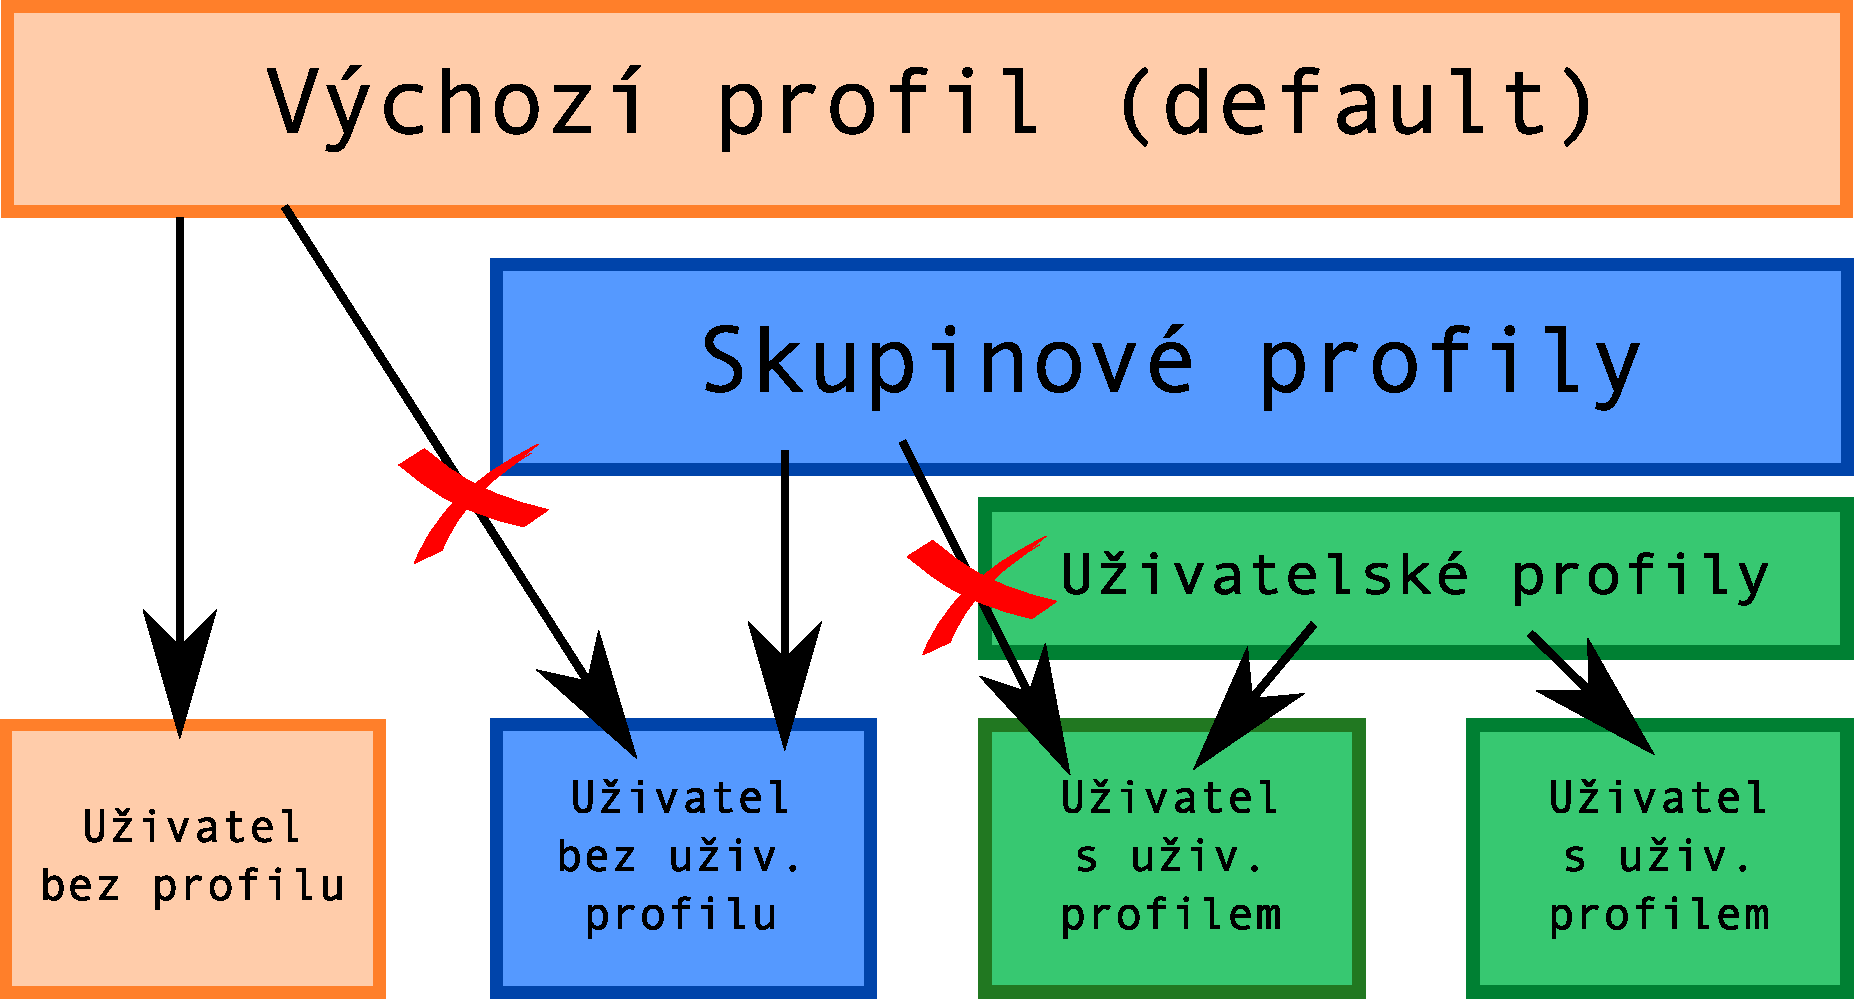
\includegraphics[width=8.5cm]{obrazky/profily.pdf}
    \caption{Aplikace Kiosk profilů}
    \label{fig:konv_profily}
\end{figure}

Problémem řešení je~zejména nemožnost reprezentace vlastnosti nezměnitelnosti z~KConfigu v~plném rozsahu. Je sice možné nezměnitelnost zpracovávat v~rámci skupinových profilů, ale systém jako celek neumožní zvenku zjistit, jestli je~nějaké omezení nezměnitelné. Z~pohledu rozhraní KAuthorized jsou tak nezměnitelné všechny akce uložené v~PolicyKitu. Jedinou možností jak docílit toho, aby byla změnitelná je~nezanést ji do PolicyKitu. Pak ale není možné s~nimi v~něm pracovat. Když je~jednou akce jako \cppc{action/help} pro ukázání menu s~nápovědou zanesena do KAuthu, ztrácí nad ní uživatel kontrolu a~nemůže tak menu schovat. Toto je~bohužel při způsobu jakým je~KAuth navržen nevyhnutelné.

% svn://svn.kde.org/home/kde/trunk/extragear/base/polkit-kde-1/
\subsection*{Integrace KAuth do KAuthorized}
KAuth nabízí několik možností, jak autorizovat akci. V~zásadě se~jedná o~různé metody třídy \cppc{KAuth::Action}, mající mírně odlišný význam. Prvním metodou je~\cppc{execute()}. Tato metoda je~uvedena v~příkladu \cite{KAuthusage} a~je určena pro jednorázové blokující provedení akce. Pokud je~to potřeba, uživatel je~požádán o~autentizaci. Metoda má podle \cite{KAuthusage} fungovat i~bez přítomnosti pomocníka. \cppc{execute()} má také asynchronní verzi.

Další metodou je~\cppc{authorize()}. Tato metoda je~určena pro získání autorizace pro akce před tím, než by byla akce provedena. Má být používána ostatními metodami třídy \cppc{KAuth::Action}. Metoda podobně jako \cppc{execute()} může od~uživatele vyžadovat autentizaci. Třetí metodou je~\cppc{status()}. Tato metoda je~podobná \cppc{execute()}, ale v~případech, kdy by byla vyžadována autentizace pouze o~této skutečnosti informuje.

Ze všech uvedených metod je~tedy nejvhodnější \cppc{status()}. Po konverzi z~Kiosk profilů totiž nevznikají akce pro jejichž autorizaci by bylo nutné se~autentizovat. Rozhraní KAuthorized jsem tedy doplnil o~překlad původních názvů akcí z~Kiosku do~formy přijatelné KAuthem a~volání metody status(). Pokud KAuth nezná autorizovanou akci nebo typ dat, je~místo něj použit KConfig.

\section{Testování}
Téměř okamžitě po implementaci jsem narazil na první problém. Program, který používá upravené rozhraní KAuthorized totiž po čase přestane reagovat, společně s~PolicyKit démonem. Při integraci KAuthu do rozhraní KAuthorized, které je~využíváno téměř každým programem v~KDE je~objem dotazů o~několik řádů vyšší, než když je~KAuth normálně používán. Chyba v~podstatě umožňuje přihlášenému uživateli provést DoS\footnote{Denial of Service} útok na PolicyKit. PolicyKit démon navíc běží jako systémová služba, což znamená, že PolicyKit je~nefunkční pro všechny uživatele systému.

Pro zjištění kde je~chyba jsem vytvořil jednoduchý test kauthDoS. Ten v~nekonečném cyklu volá \cppc{KAuth::Action::status()} a~v~pravidelných intervalech vypisuje hlášení. Když program přestane vypisovat, znamená to, že došlo k~chybě. Zdrojový kód nástroje je~v~\cppc{kdelibs/kdecore/auth/kauthDoS.cpp}.

Démon polkitd a~program kauthDoS byly spuštěny v~debuggeru gdb a~byly získány \uv{backtrace} z~obou programů (výpisy v~přílohách \ref{btrac1} a~\ref{btrac2}). Problém vzniká během komunikace jednotlivých částí PolicyKitu. Chybu jsem ohlásil jeho autorovi (David Zeuthen) v~mailing listu PolicyKitu \cite{bugrepmailinglist} a~nedočkal se~odpověďi, i~když je~tento mailing list uveden jako místo kam se~mají chyby PolicyKitu hlásit.

Provedl jsem tedy druhý pokus o~nahlášení chyby a~přitom implementoval test podobný KAuthDoS, ale závisející pouze na PolicyKitu.
Chyba byla hlášena do bugtrackeru PolicyKitu \cite{bugreptracker}, ale setkala se~s~nepochopením ze strany autora.

Jako dočasné řešení jsem do implementace v~rozhraní KAuthorized přidal test na proměnnou prostředí \cppc{KDE_KIOSK_USE_KAUTH}. Pokud je~nastavena na \cppc{YES}, použije se~jako zdroj autorizací KAuth, jinak se~použije KConfig.

Při hledání chyby jsem narazil na druhý problém v~PolicyKitu, kdy každý požadavek na autorizaci způsoboval zahození celé databáze autorizací a~jeji opětovné načtení z~konfiguračních souborů. Tato chyba byla opravena, viz bugtracker: \cite{smallbugrep}.

\subsection*{Testování implementace}
K~testování implementace jsem vytvořil jednoduchý program, který kontroluje, jestli získá použitím KAuth a KConfig rozdílné výsledky pro stejnou akci. Jde o~jednoduché volání funkce \cppc{authorize()} z~rozhraní \cppc{KAuthorized} kombinované s~použitím proměnné prostředí \cppc{KDE_KIOSK_USE_KAUTH}. Zdrojem názvů akcí je~statický seznam řetězců obsažený ve zdrojovém kódu programu. Ten obsahuje stejné názvy akcí jako statický .actions soubor použitý KAuthem na generování nastavení pro PolicyKit. Zdrojový kód programu lze nalézt v~\cppc{kdelibs/kdecore/auth/integtest.cpp} a~výsledný spustitelný soubor má název \cppc{integtest}.

Postup testování je~takový, že se~vytvoří určitá množina profilů, které se~přiřadí uživateli nebo skupinám. Dále se~spustí implementovaný konvertor nastavení \cppc{kioskpklaconvert} a~poté nástroj \cppc{integtest}. Pomocí tohoto nástroje jsem testoval několik možných scénářů:

\begin{itemize}
\item Pouze výchozí profil (uživatel nemá přiřazené žádné profily).
\item Výchozí profil plus dva skupinové profily, kdy v~prvním skupinovém profilu jsou podorované akce nastaveny jako nezměnitelné. Všechny profily mají jiné nastavení. Je očekáváno, že výsledné autorizované akce budou identické s~těmi v~prvním skupinovém profilu a~výchozí profil nebude mít žádný efekt.
\item Kombinace skupinového a~uživatelského profilu s~jiným nastavením a~bez nezměnitelnosti. Očekává se, že bude efektivní pouze uživatelský profil.
\item Uživatelský profil bez nezměnitelnosti plus jiné nastavení v~domovském adresáři uživatele. Očekává se, že bude v~případě použití KAuth efektivní uživatelský profil a~v~případě použití KConfig nastavení v~domovském adresáři (tedy, že KAuth nepodporuje nezměnitelnost).
\end{itemize}

Všechny testy proběhly podle očekávání.

Dále jdem vytvořil jednoduchý test na ověření funkčnosti KAuth: kauthtest. Ten testuje reakci KAuth na požadavek o~autorizaci čtyř akcí. Jedna je~vždy autorizována, jedna není autorizována nikdy, jedna vyžaduje přihlášení uživatele a~jedna neexistuje. Tento nástroj byl použit k ověření funkčnosti KAuth během implementace změn v~něm.

\section{Návrh dalšího postupu}
Výše byly popsány vybrané části rozhraní KAuthorized a~KAuth a~také jejich integrace. Nyní následuje návrh řešení v~nich nalezených nedostatků a~také návrh na jejich rozšíření. V~prvé řadě je~potřeba opravit zmíněnou bezpečnostní chybu v~PolicyKitu. 

Dále je~potřeba rozšířit KAuth:
\begin{enumerate}
\item Je potřeba, aby uměl hlásit, pokud autorizovaná akce není známa -- a~to pro všechny podporované autorizační systémy. Toto jsem pro účely práce udělal a~otestoval pro metodu \cppc{status()} a~PolicyKit1. Ideální by bylo integrovat vyhledání akce do~konstruktoru třídy \cppc{KAuth::Action} a~vracet pak výsledek pomocí volání její metody \cppc{isValid()}.
\item KAuth musí umět nejen ověřovat a~spouštět akce, ale také měnit oprávnění k~těmto akcím pro uživatele a~skupiny. Zde je~zatím k~dispozici pouze KControl modul pro PolicyKit v~balíku policykit-kde-1 a~s~ním spojený pomocník na bázi polkit-qt-1, ale ten je~zaměřen pouze na uživatele KContorol modulu a~není nijak do KAuthu integrován.
\item Mělo by také být možné přidávat nové akce. To znamená, že by se~nemusely do systému instalovat statické soubory s~definicemi akcí.
\item V~neposlední řadě by také mělo jít doplnit podporu nezměnitelnosti do rozhraní KAuth. To vyžaduje další změny v~knihovně polkit-qt, která je~využita mezi KAuthem a~samotným PolicyKitem.
\end{enumerate}

Bod 1 nezávisle implementoval Dario Freddi, ale implementace způsobuje množství chyb typu segmentation fault při použití KAuth z~rozhraní KAuthorized. Na vině je~to, že KAuthorized je~využíván dříve, než jsou všechny části aplikace inicializovány a~takto upravený KAuth na nich závisí. V~zájmu funkčnosti řešení jsem tyto změny odstranil. Pokud má být KAuth skutečně integrován do KAuthorized, bude potřeba tento problém korektně vyřešit.

Body 2 a~3 by bylo možné realizovat jakožto pomocníky a~přidat do systému KAuth rozhraní, které by umožnilo s~nimi pracovat.

Díky omezením ze strany KAuthu a~nalezeným chybám je~bohužel integrace KAuthu do Kiosku pouhým experimentem. Oba systémy jsou totiž velmi rozdílné v~některých kritických bodech a~KAuth nikdy nemůže plně nahradit flexibilitu KConfigu. Jedinou výhodou použití KAuth je~tak jen skrytí nastavení před uživateli, a~to pouze v~případě, že by se~podařilo dohledat všechny akce v~Kiosku použité, převést veškeré Kiosk profily na nastavení KAuth a~následně je~buď odstranit ze systému, nebo k~nim omezit přístup. Omezení přístupu je~všek problematické, protože omezení akcí a~zdrojů v~Kiosk profilech může být promícháno s~normálním nastavením aplikací. Pozitivními výsledky integrace jsou tak jen nalezené a~opravené chyby.

KAuth by bylo lepší použít k~tomu, k~čemu byl určen. Tedy k~oddělení částí aplikací, které vyžadují administrátoská práva od~těch částí, které je~nevyžadují. Ne však jako úložiště nastavení.

Některé změny implementované v~KDE-Libs pro účely integrace KAuth a~Kiosku by však bylo možné bez problémů začlenit. Zde se~jedná zejména o~načítání omezení zdrojů dat z~Kiosk profilů, které předtím nebylo funkční.

Kiosk jako celek je~bohužel jednou z~méně udržovaných částí KDE-Libs a~určitá část nastavitelných omezení je~zcela neefektivní. Další postup by tedy měl spíše směřovat k~obnovení funkčnosti jednotlivých omezení akcí a~zdrojů dat v~Kiosku.  Ne všechny jeho části přežily přechod z~KDE~3 na KDE~4 bez úhony. Prvním krokem by mohlo být odstranění zdvojení funkce pro autorizaci akcí cppc{authorize()} a~\cppc{authorizeKAction()}.

\chapter{Nástroj KioskTool}
Tato kapitola se~zabývá portem nástroje KioskTool z~KDE~3 na KDE~4. Nástroj KioskTool slouží k~jednoduchému vytváření, nastavování a~přiřazování Kiosk profilů. V~současné době existuje ve dvou verzích. Starší verze pro prostředí KDE~3 a~novější, ale nedokončený port pro KDE~4. Funkce verze pro KDE~3 jsou pro názornost ilustrovány snímky z~okna programu. V~kapitole je~čerpáno ze knih \cite{StarchQt4,Ezust} a online dokumentace ke knihovně Qt\cite{nokiaQt}.

\section{KioskTool v~KDE~3}
\begin{figure}[h]
\centering
\begin{tabular}{c c}
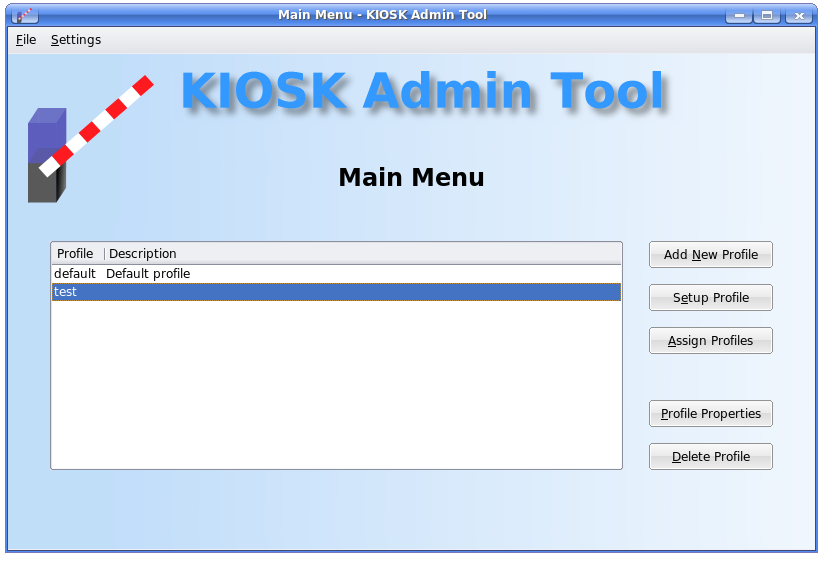
\includegraphics[width=7.2cm ,keepaspectratio]{obrazky/KioskToolKDE3/uvodni_obrazovka.png}&
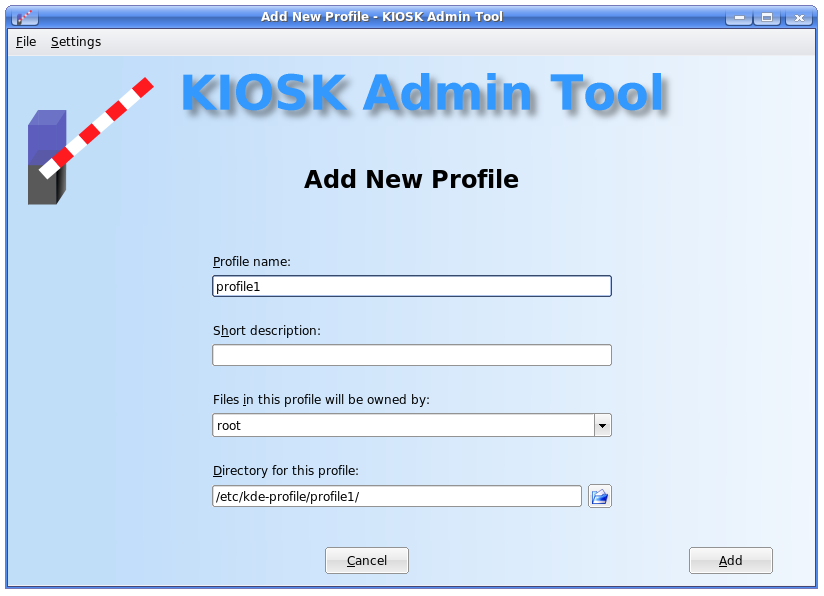
\includegraphics[width=7.2cm ,keepaspectratio]{obrazky/KioskToolKDE3/novy_profil.png}\\
(a)&(b)\\
\end{tabular}
\caption{Úvodní obrazovka programu (a) a dialog pro vytvoření nového profilu (b).}
\label{fig_6}
\end{figure}

Úvodní obrazovka \ref{fig_6}a ukazuje seznam profilů s~jejich popisem, lištu s~menu a~tlačítka pro manipulaci s~profily. Velmi chybí možnost vytvoření kopie již existujícího Kiosk profilu.

Dialog \ref{fig_6}b pro vytvoření nového profilu je~poměrně jednoduchý. Umožňuje nastavit název a~popis profilu a~dále který uživatel bude vlastnit složku s~profilem (bude mít přístup pro zápis) a~kde bude profil uložen.

\begin{figure}[ht]
\centering
\begin{tabular}{c c}
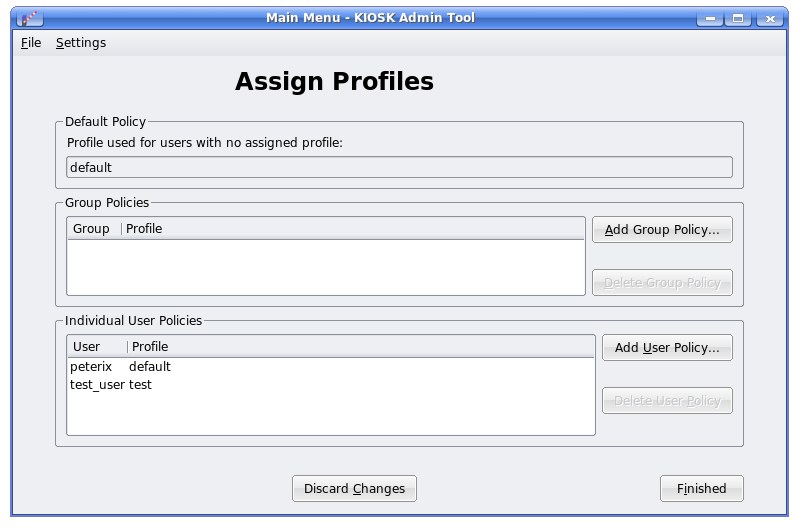
\includegraphics[width=7.2cm ,keepaspectratio]{obrazky/KioskToolKDE3/prirazeni_profilu.png}&
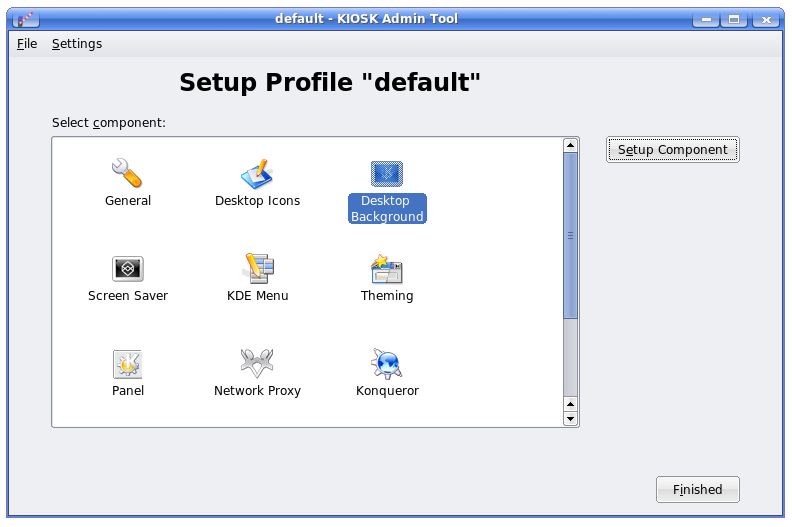
\includegraphics[width=7.2cm]{obrazky/KioskToolKDE3/seznam_komponent.png}\\
(a)&(b)\\
\end{tabular}
\caption{Dialog pro přiřazení profilů (a) a dialog pro úpravu profilu (b).}
\label{fig_7}
\end{figure}

Dialog pro přiřazení Kiosk profilů skupinám a~uživatelům na obrázku \ref{fig_7}a je~až příliš jednoduchý. Když má uživatel přiřazen svůj vlastní profil, nevztahují se~na něj profily pro skupiny kterých je~členem. Toto není v~programu nijak poznat. Zde by bylo vhodné, kdyby program poskytoval nějaký pohled, který by ukazoval všechny profily efektivní pro uživatele. Výchozí Kiosk profil takto zvýrazněn je.

Na obrázku \ref{fig_7}b je~dialog pro úpravu profilu. Nastavení je~rozděleno na jednotlivé komponenty. Je možné z~něj navíc spouštět další části systému KDE a~tak docílit toho, že KioskTool může využít již existující funkcionalitu. Není proto nutné znovu implementovat něco, co již funguje a~uživatel pro nastavení Kiosk profilů používá stejné nástroje jako pro normální nastavení.

\begin{figure}[h]
    \centering
    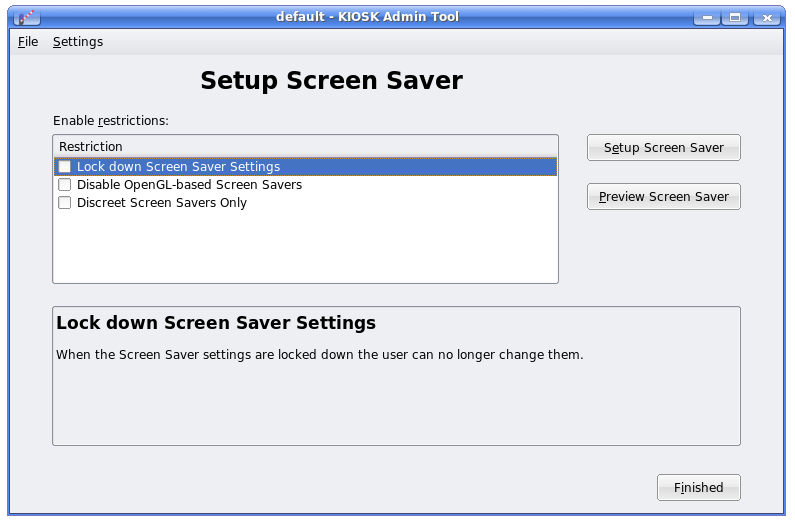
\includegraphics[width=10cm]{obrazky/KioskToolKDE3/ukazka_komponenty.png}
    \caption{Dialog jedné komponenty nástroje}
    \label{fig:kt3_nast_komp}
\end{figure}
Na obrázku \ref{fig:kt3_nast_komp} je~vidět jak taková komponenta vypadá. Uživatel může zamknout pozadí plochy a~ukázat si náhled tohoto pozadí (náhled ve smyslu, že se~pozadí plochy dočasně zamění).

I~při krátké době nutné na seznámení s~nástrojem (KioskTool 1.0 v~Kubuntu 9.04) jsem narazil na fatální chyby, kdy se~bez zjevného důvodu zhroutil. Není tedy možné se~spolehnout na korektnost kódu.

\section{KioskTool v~KDE 4}
Port nástroje do KDE~4 již existuje, i~když je~nedokončený a~dá se~říci opuštěný. Uživatelské rozhraní se~příliš nezměnilo co se~týče struktury, pouze ztratilo původní vzhled, viz. obrázek \ref{fig:kt4_uvod}. Původní nastavení pomocí velkého XML souboru bylo odstraněno a~nahrazeno mnoha menšími soubory (používá se~KConfig). To má za účel umožnit ostatím autorům napsat si pro své aplikace rozšíření. Nástroj však ztratil většinu svých starých vlastností, schopnost spouštět KControl moduly a~náhledy, již zmíněný vzhled a~získal několik dalších chyb.

\begin{figure}[h]
    \centering
    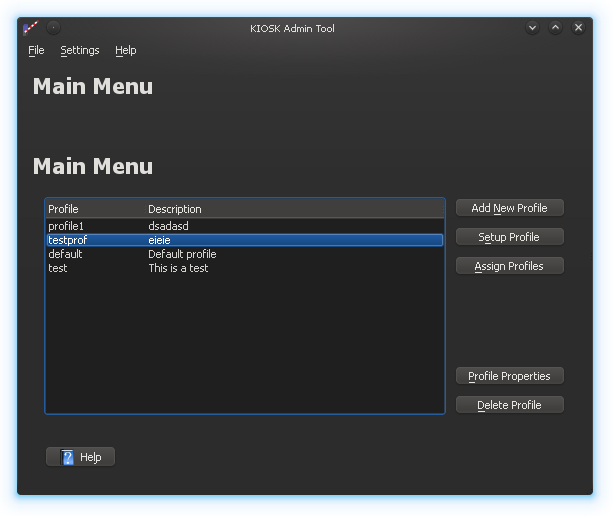
\includegraphics[width=10cm]{obrazky/KioskToolKDE4/kiosktool_kde4.png}
    \caption{Uživatelské rozhraní se~od~verze z~KDE3 příliš nezměnilo}
    \label{fig:kt4_uvod}
\end{figure}

\paragraph{Funkční popis}
Aplikace KioskTool se~skládá z~několika základních komponent a~využívá grafické rozhraní navržené pomocí nástroj Qt Designer (části rozhraní jsou specifikovány v~.ui souborech, ze kterých se~při kompilaci generuje kód). Vzhled je~tedy alespoň z~pohledu programátora částečně oddělen od~funkce programu. Grafické prvky programu však přímo obsahují data se~kterými se~pracuje. Není využito návrhového vzoru MVC\footnote{Model-View-Controller}.

Při startu programu jsou nejdříve vytvořeny základní komponenty \cppc{KAboutData} a~\cppc{KApplication} a~hlavní komponenta grafického rozhraní \cppc{KioskGui}. Ta je~zobrazena. Potom je~nastartováno vyhodnocování událostí.

Komponenta \cppc{KioskGui} je~odvozena od~třídy \cppc{KXmlGuiWindow} a načítá část svého vzhledu z~.rc souboru viz. výpis  \ref{listing:guirc} ve formátu XML.
\begin{mylisting}
\caption{kiosktoolui.rc}
\label{listing:guirc}
\begin{lstlisting}[language=XML]
<?xml version="1.0"?>
<!DOCTYPE gui SYSTEM "kpartgui.dtd">
<gui name="kioskgui" version="3.1">
<MenuBar>
 <Menu name="file">
    <Action name="upload_all"/>
 </Menu>
</MenuBar>
</gui>
\end{lstlisting}
\end{mylisting}

\cppc{KioskGui} potom vytváří instance tříd \cppc{KioskRun} a~\cppc{MainView}. \cppc{KioskRun} je~pouhou obálkou nad souborem funkcí různého určení a~je používána pro většinu manipulace s~profily a~spouštění dalších programů. \cppc{MainView} pak určuje vzhled celého programu. Je to třída generovaná z~.ui souboru, obsahuje dvě úrovně nadpisů, tři tlačítka která mění význam podle kontextu a~objekt typu \cppc{QStackedWidget}, který je~určen pro zobrazení aktuální stránky. Při startu je~to stránka se~seznamem profilů (\cppc{PAGE_PROFILE_SELECTION}).

Přechod mezi stránkami je~prováděn pomocí metody \cppc{selectPage(enum page)}, volané v~reakci na akce uživatele a~lze v~hrubých obrysech popsat pomocí stavového automatu na diagramu \ref{fig:kioskstates}. Návrat z~vyvolané karty je~možný buď pomocí metody \cppc{finishedPage()}, která uloží provedené změny, nebo metody \cppc{discardPage()}, která změny zahazuje.

\begin{figure}[h]
    \centering
    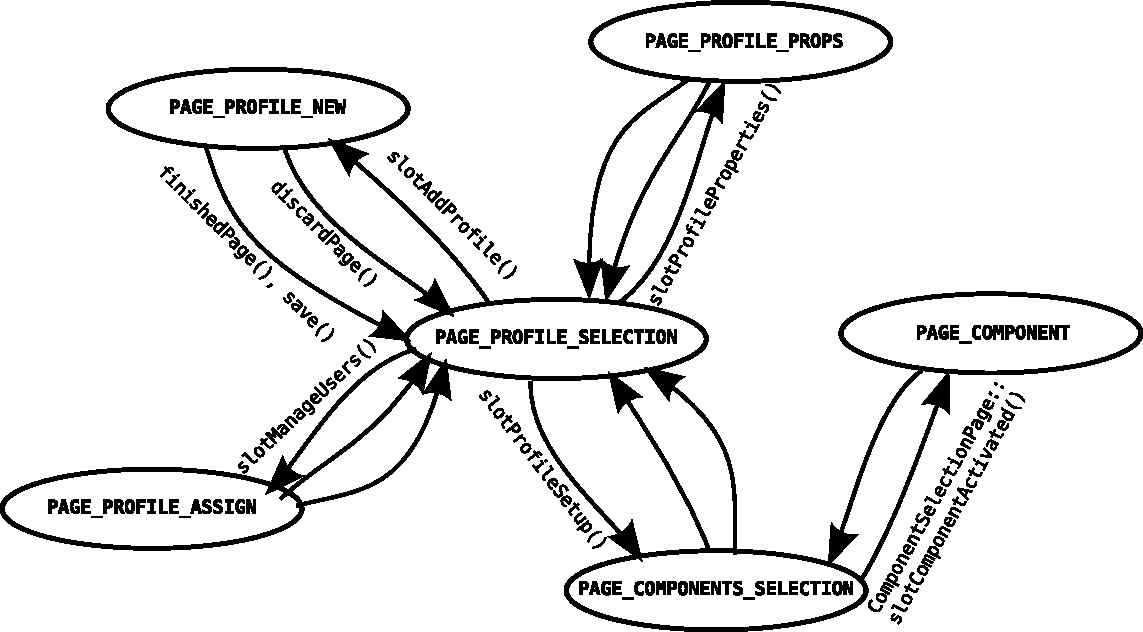
\includegraphics[width=10cm]{obrazky/stated.pdf}
    \caption{Stavy grafického rozhraní aplikace KioskTool}
    \label{fig:kioskstates}
\end{figure}

Ve stavech \cppc{PAGE_PROFILE_NEW} a~\cppc{PAGE_PROFILE_PROPS} je~použito stejné grafické rozhraní. Jednou pro vytvoření nového profilu, podruhé pro změny v~něm.\linebreak \cppc{PAGE_PROFILE_ASSIGN} je~stav, ve kterém je~aktivní stránka pro přiřazení profilů uživatelům a~skupinám. Ve stavu \cppc{PAGE_COMPONENTS_SELECTION} je~načten profil a~je zobrazena stránka se~seznamem komponent pro stav \cppc{PAGE_COMPONENT}. Seznam komponent je~určen konfigurací načtenou ze souborů používajících formát KConfig.

Je zřejmé, že způsob jakým je~vytvořeno grafické rozhraní přímo určuje funkci programu. Přechod na stránku se~seznamem komponent zapříčiní otevření profilu. Návrat na hlavní stránku se~seznamem profilů pak způsobí jeho uložení. Platí to i~naopak -- technická omezení kladená na některé funkce programu se~odrážejí v~návrhu jeho grafického rozhraní. Například program nemůže upravovat více jak jeden profil, protože ve třídě \cppc{KioskRun} nastavuje pro spuštění KConfig modulů proměnné prostředí a~kopíruje profil do~dočasného umístění, kde ho může případná spouštěná aplikace měnit. Proto stavový automat a~přechody mezi stránkami.

\section{Návrh nového uživatelského rozhraní}
Zde je~použit nástroj QtDesigner pro navržení vzhledu uživatelského rozhraní.

V~prve řadě bude sloučeno několik karet určených pro správu profilů do jednoho celku a~funkce editace profilů bude oddělena. Namísto stránek a~stavových automatů bude mít část pro správu profilů několik záložek. Zůstanou tlačítka s~akcemi po stranách, ale uživatel bude mít mnohem větší přehled o~celkovém stavu Kiosku.

\begin{figure}
\centering
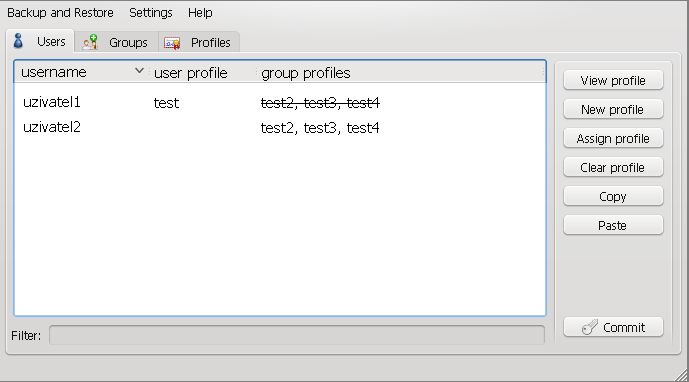
\includegraphics[width=10cm, keepaspectratio]{obrazky/navrh-usersz.png}
\caption{Karta pro uživatele}
\vspace{5 mm}
\label{fig:kt4_newusers}
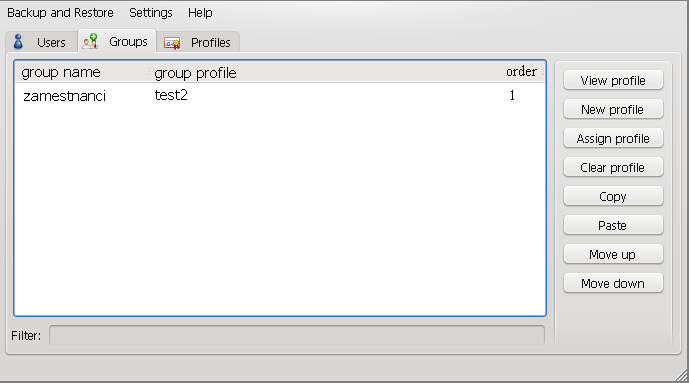
\includegraphics[width=10cm, keepaspectratio]{obrazky/navrh-groupsz.png}
\caption{Karta pro skupiny}
\label{fig:kt4_newgroups}
\end{figure}

Na obrázku \ref{fig:kt4_newusers} je~program s~otevřenou kartou pro pohled na uživatele. Menu Settings bude rozšířeno o~možnost spustit konvertor na nastavení KAuth implementovaný v~předchozí kapitole. Většinu plochy programu zabírá pohled na seznam uživatelů a~k~nim přiřazených uživatelských a~skupinových profilů. Pokud má uživatel přiřazen jak uživatelský, tak skupinové profily, je~zde fakt, že jsou ty skupinové profily neefektivní graficky zvýrazněn.

V~seznamu po pravé straně je~několik pro KioskTool nových akcí. Akce \uv{Assign Profile} slouží k~přiřazení existujícího profilu uživateli a~bude otevírat jednoduchý modální dialog se~seznamem existujících profilů. \uv{Clear Profile} odebere uživateli jeho profil. Copy a~Paste slouží ke kopírování stejného nastavení uživatelského profilu mezi uživateli.

Karta se~skupinami na obrázku \ref{fig:kt4_newgroups} je~podobná kartě pro uživatele, zobrazuje však skupiny, jim přiřazené skupinové profily a~pořadí skupin zde odpovídá pořadí zpracování skupinových profilů v~systému Kiosk. K~seznamu akcí z~karty s~uživateli jsou přidány akce \uv{Move up} a~\uv{Move down} pro změnu pořadí skupin.

\begin{figure}[h]
    \centering
    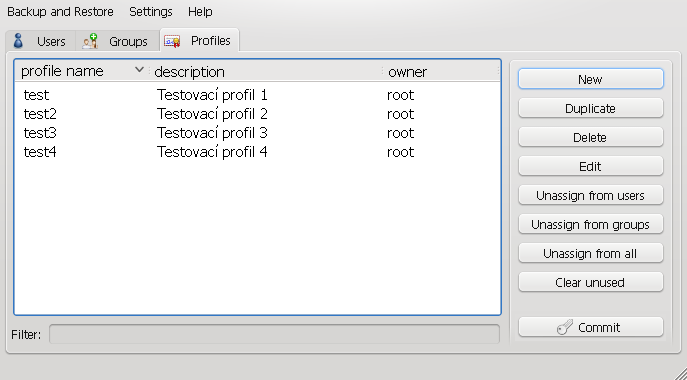
\includegraphics[width=13cm]{obrazky/navrh-profiles-fixd.png}
    \caption{Karta pro profily}
    \label{fig:kt4_newprofiles}
\end{figure}

Záložka s~profily na obrázku \ref{fig:kt4_newprofiles} obsahuje seznam profilů a~akce pro práci s~nimi. V~pořadí odshora vytvoření nového profilu, kopie již existujícího profilu, smazání profilu, úpravu profilu, akci pro otevření původní karty s~vlastnostmi profilu jako modální dialog, a~dále akce pro zrušení přiřazení profilů pro uživatele, skupiny a~obojí zároveň. Seznam je~zakončen akcí pro smazání všech nepoužívaných profilů.

Všechny záložky také mají akci pro uložení změn \uv{Commit}. Její použití vyžaduje administrátorská práva.

\section{Implementace}
Hlavní část implementace spočívá v~rozdělení třídy \cppc{KioskGui} na dvě části. První část je~použita pro zobrazení a~obsluhu nového hlavního okna. Je~z~ní odstraněn původní stavový automat a~rozhraní na~bázi \uv{výměny karet} je~nahrazeno vytvářením modálních dialogových oken. Druhá část si zachovává charakter původní třídy \cppc{KioskGui} a~je použita k nastavování Kiosk profilů.

Implementace nového uživatelského rozhraní spočívá v~odstranění původního rozhraní na~bázi třídy \cppc{KioskGui}, použití navrženého grafického rozhraní v~této třídě a~implementaci modelů, které slouží jako zdroj dat pro jednotlivé pohledy.

\begin{figure}[h]
    \centering
    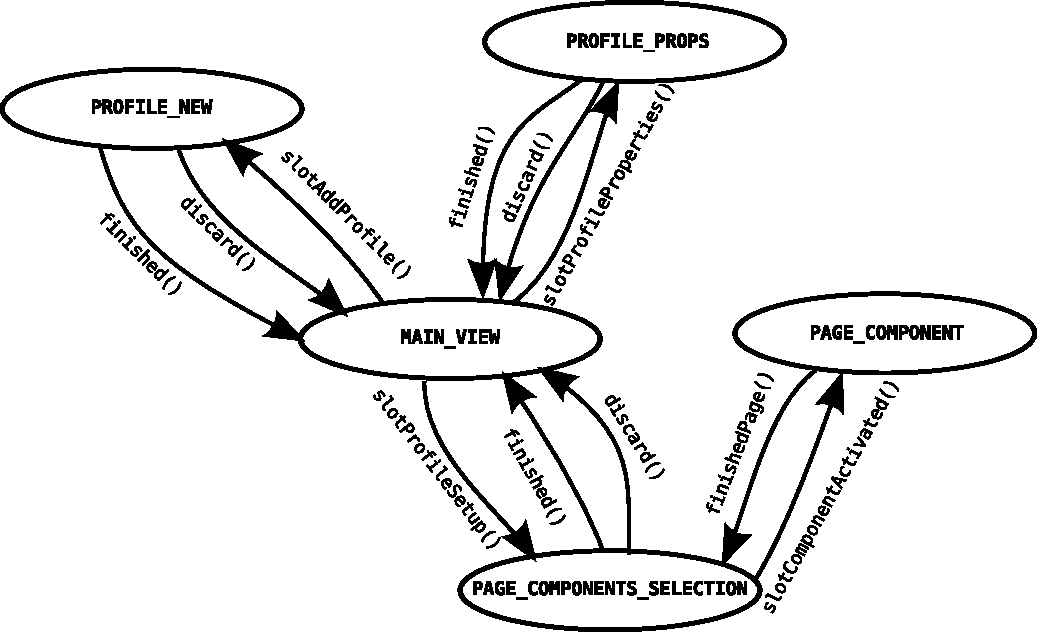
\includegraphics[width=10cm]{obrazky/stated-new.pdf}
    \caption{Stavy grafického rozhraní aplikace KioskTool s~úpravami}
    \label{fig:kioskstatesnew}
\end{figure}

Přechod mezi stavy programu je~opět možné modelovat stavovým diagramem, viz. obrázek \ref{fig:kioskstatesnew}. Oproti původnímu diagramu je~odstraněn stav pro přiřazování vybraného profilu uživatelům a~skupinám, protože je tato funkce součástí nového hlavního okna (\cppc{MAIN_VIEW}). Všechny přechody ze stavu \cppc{MAIN_VIEW} místo výměny karet otevírají modální dialogy.

Jediným typem vstupu od~pohledů bude výběr jedné položky. Tlačítka po pravé straně slouží ke spouštění akcí upravujících stav modelů. Akce \uv{Commit} pak způsobí uložení změn.

Pohledy v novém uživatelském rozhraní jsou odvozeny od~třídy \cppc{QTreeView}, protože podporuje zobrazení více sloupců a~jejich záhlaví. Pro správu profilů je~využita třída \cppc{KioskRun}, která je také zdrojem dat pro modely jednotlivých pohledů. Pohled na uživatele zobrazuje všechny uživatele systému. Podobně pohled na skupiny zobrazuje všechny skupiny. Do hlavního menu byla dále přidána akce pro konverzi Kiosk profilů na nastavení pro PolicyKit. Ta používá konvertor implementovaný v~předchozí kapitole. Počet akcí u~jednotlivých pohledů byl oproti návrhu redukován. Odpadají tak akce pro prohlížení stávajících a~vytváření nových profilů u~pohledu na~uživatele a~skupiny.

Řešení editace Kiosk profilů se v~zásadě nijak nezměnilo. Původní třída \cppc{KioskGui} byla zkopírována a~využita jako editor profilů pod jménem \cppc{ProfileEditGui}. Počet stavů mezi kterými se~může třída pohybovat je~výrazně menší, než u~původního \cppc{KioskGui}. Buď je ve stavu, kdy se zobrazuje seznam komponent profilu, nebo zobrazuje jednu z~komponent specifikovaných v~souborech s nastavením programu. Byly z~ní odstraněny stavy související se správou profilů.

Zbytek programu se, až na kosmetické úpravy jednotlivých karet nyní převedených na modální dialogy, nemění.

\subsection*{Další možný postup}
V~této fázi je~nástroj KioskTool použitelný pro nastavení omezení akcí a~byly v~něm díky provedeným změnám odstraněny chyby. Editace profilů by však stále mohla být řešena lépe. Díky oddělení správy profilů je možné relativně jednoduše nahradit stávající editor. Například by mohl být integrován nástroj KConfigEditor\cite{KConfigEditor}, pro ilustraci uvedený v~podobě snímku obrazovky \ref{fig:kconfeditor}.

KConfigEditor používá rozšíření systému KConfig o~deklarace klíčů a~jejich typů pomocí systému KConfigXT. Ten je~zpravidla používán k~vygenerování dialogů pro nastavení programů. Soubory s~nastavením KConfigXT se~instalují společně s~programy a~lze jich tedy využít právě v~takovémto editoru nastavení. Program je~podobně jako původní KioskTool napsán pro KDE~3 a~dosud nebyl proveden žádný pokus o~jeho port do~KDE~4. Integrace tohoto nástroje a~rozšíření a~oprava KConfigXT souborů by vedly k~vcelku elegantnímu řešení problému úpravy Kiosk profilů. KioskTool by pak mohl sloužit i~k~změnám nastavení v~domovské složce přihlášeného uživatele, které by jinak musel uživatel dělat v obyčejném textovém editoru.

\begin{figure}[h]
    \centering
    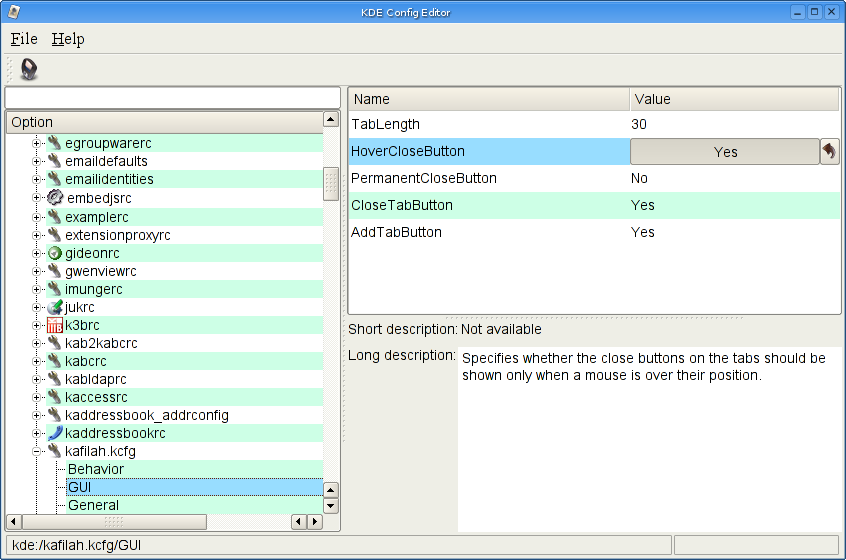
\includegraphics[width=10cm]{obrazky/kconfigeditor1.png}
    \caption{Ukázka programu KConfigEditor. Převzato z~\cite{KConfigEditor}.}
    \label{fig:kconfeditor}
\end{figure}


\chapter{Závěr}
Ve druhé kapitole byly popsány technologie a~rozhraní na kterých je~dále stavěno. Zejména Kiosk, KConfig, KAuth, KAuthorized a~PolicyKit. Kapitola také popisuje základy řízení přístupu k~souborům v~systému Linux.

Ve třetí kapitole byla navržena a~implementována integrace rozhraní KAuth a~KAuthorized. Během návrhu a~implementace byly odkryty některé závažné nedostatky v~KAuth a~rozhraní PolicyKit, nad kterým je~postaven. Zejména Denial of~Service útok na PolicyKit. Ten jsem objevil za pomoci implementovaného testovacího nástroje kauthDoS. Integrace má spíše experimentální charakter a~jejím hlavním přínosem jsou objevené a~opravené chyby v~integrovaných rozhraních. Začlenění tohoto celku do hlavní vývojové větve balíku KDE-Libs tak není z~praktických a~bezpečnostních důvodů vhodné, i~když je kód v~podobě patche pro takové začlenění připraven. Ve třetí kapitole jsou splněny body zadání 2,3~a~5.

Dále byl implementován nástroj kioskpklaconvert a~KAuth pomocník kioskpklahelper. Ty umožňují konvertovat omezení akcí a~zdrojů z~KConfigu do nastavení PolicyKit Local Authority. Byly také implementovány testy ověřující funkčnost řešení.

Kapitola 4 popisuje původní verzi nástroje KioskTool, již existující port do KDE~4 a~navrhuje pro něj nové grafické rozhraní. Je také stručně popsána implementace změny grafického rozhraní a~způsob interakce nástroje KioskTool s~rozhraním KAuth integrovaným do Kiosku (je použit konvertor implementovaný ve třetí kapitole). Tím je~také splněn čtvrtý bod zadání.

V~příloze B jsou informace o~umístění zdrojových kódů, obsahu přiloženého datového nosiče a~instalaci a~zprovoznění KDE~4 kompilací ze zdrojového kódů.

%=========================================================================
\appendix
\chapter{Vymezení pojmů}\label{pojmySeznam}
\begin{description}
\item[KDE] je~komunita vývojářů pracujících na tzv. KDE Software Compilation.
\item[KDE SC,] nebo také KDE Software Compilation zahrnuje veškeré projekty KDE, které mají jednotný vývojový cyklus.
\item[KAuth] je~rozhraní nad autorizačním řešením jako je~například PolicyKit.
\item[KConfig] je~systém pro ukládání a~načítání nastavení v~KDE SC.
\item[Kiosk] je~framework sdružující aplikační rozhraní KAuthorized, některé vlastnosti KConfigu a~postup načítání konfigurace obecně.
\item[Kiosk profil] je~přiřazený uživateli nebo skupině uživatelů. Má vyšší prioritu než normální uživatelská nastavení KDE, ale nižší než globální systémové nastavení.
\item[KioskTool] je~aplikace pro správu Kiosk profilů. V~KDE 3 umožňovala jednoduše nastavit některé aspekty Kiosku/KConfigu bez nutnosti měnit profily ručně.
\item[KAuthorized] je~tenké rozhraní nad KConfigem/Kioskem umožňující dotazování, zda jsou některé typy akcí povoleny.
\item[KConfigXT] je~systém pro uložení metadat pro systém KConfig. Popisuje klíče použité v~jednotlivých programech a~jejich typy.
\item[KControl modul] je~modulem pro nastavení určité části KDE SC. Například rozložení klávesnice, vzhledu oken, apod.
\item[PolicyKit] je~starší verze autorizačního rozhraní dostupná v~Linuxu.
\item[PolicyKit1,] nebo také \uv{polkit-1} je~jeho novější verze. Právě ta je v~práci použita.
\item[PolicyKit autorita] je~centrálním prvkem systému PolicyKit. Slouží pro uložení autorizačních dat.
\item[PolicyKit Local Authority] je~výchozí implementace PolicyKit autority. Používá textové soubory.
\item[polkit-qt] je~soubor knihoven obalující PolicyKit.
\item[polkit-kde] je~nadstavba nad polkit-qt pro prostředí KDE SC. Implementuje autentizačního agenta a~KControl modul pro práci s~autorizacemi.
\item[polkitd] je~systémová služba PolicyKitu a~implementuje PolicyKit autoritu.
\item[Authorization Services] je~obdoba PolicyKitu pro operační systém Apple OSX.
\item[Qt] je~balík knihoven v~jazyce C++, které jsou použity jak základ pro KDE~SC.
\item[QtDesigner] je~program pro vizuální návrh uživatelského rozhraní programů založených na knihovnách Qt.
\end{description}
%=========================================================================
\chapter{Instrukce pro sestavení a~obsah přiloženého média}
\section*{Instalace - Integrace KAuth do KAuthorized}
Kód práce je~v~době odevzdání založen na SVN revizi 1154555. Je tedy nutné získat právě tuto revizi. V~opačném případě se~nemusí podařit patch pro KDE-Libs aplikovat, nebo mohou změny v~novějších revizích změnit chování implementace. Kód z~třetí kapitoly \textbf{VYŽADUJE}, aby byl v~systému nainstalován PolicyKit1. Konvertor totiž funguje s novější verzí, která není se staršími verzemi PolicyKitu kompatibilní. Aktuální verze PolicyKitu v~době odevzdání je~0.96.

Sestavení KDE je~popsáno v~dokumentu, který je~dostupný na adrese \cite{KDESetup}.

Nejdříve je~potřeba vytvořit v~systému uživatele kde-devel. Dalším krokem je~nastavení jeho účtu tak, aby bylo možné sestavit a~spustit KDE~4 z~jeho domovského adresáře. Postupně je~potřeba získat a~sestavit tyto moduly: kdesupport, kdelibs, kdepimlibs a~kdebase.

Po úspěšném sestavení KDE je~nutné překopírovat registrační soubory KAuth pomocníků pro systém D-Bus a~soubory s~definicemi akcí pro PolicyKit do systémových adresářů. Bez toho nemůže KAuth fungovat. Konkrétně se~jedná o~tyto soubory:
\begin{itemize}
\item Vše z~\cppc{\$prefix/etc/dbus-1/system.d} do \cppc{/etc/dbus-1/system.d}
\item Vše z~\cppc{\$prefix/share/polkit-1/actions} do \cppc{/usr/share/polkit-1/actions}
\item Vše z~\cppc{\$prefix/share/dbus-1/system-services} do \cppc{/usr/share/dbus-1/system-services}
\end{itemize}

\noindent
\cppc{\$prefix} je~zde složka, kam se~instaluje KDE~4 zkompilované ze zdrojových kódů. V~případě použití uživatele kde-devel to bude \cppc{/home/kde-devel/kde}

Použití KAuth v~KAuthorized je~ve výchozím stavu vypnuto. K~jeho zapnutí je~potřeba v~terminálu nastavit proměnnou prostředí \cppc{KDE_KIOSK_USE_KAUTH} na hodnotu \cppc{YES}, například takto:

\cppc{\$ export KDE_KIOSK_USE_KAUTH=YES}

Všechny aplikace KDE spuštěné z~tohoto terminálu budou KAuth používat.

\section*{Instalace - KioskTool}
KioskTool by neměl vyžadovat žádné zvláštní zacházení. Není ani potřeba použít oddělený uživatelský účet kde-devel. Stačí vygenerovat buildsystém pomocí cmake, program zkompilovat a~nainstalovat.

Příklad postupu ze složky se~zdrojovým kódem, umístěné tak, aby se~do ní dalo zapisovat:
\begin{itemize}
\item \cppc{mkdir build && cd build}
\item \cppc{cmake ..}
\item \cppc{make}
\item \cppc{sudo make install}
\end{itemize}
Při použití kde-devel stačí umístit zdrojové kódy KioskTool mezi zdrojové kódy ostatních částí KDE a~sestavit je~pomocí \cppc{cmakekde}.

\section*{Obsah přiloženého média}
\begin{figure}[h!]
    \centering
    \begin{verbatim}
┬─── src ───┬─ KDELibs-patch - Patch aplikovatelný na KDE-Libs.
│           │
│           ├─ KDE           - Kopie zdrojových kódů KDE.
│           │                  (patch je již aplikován)
│           │
│           └─ kiosktool     - Zdrojový kód nástroje KioskTool.
│
├─── tex ─── ...             - Zdrojový kód pro sestavení technické zprávy.
│
└── projekt.pdf              - Elektronická kopie technické zprávy.
\end{verbatim}
\end{figure}

\chapter{Backtrace z~KAuthDoS a~PolicyKit démona}
\lstset{basicstyle=\scriptsize\ttfamily}
\begin{mylisting}
\caption{Backtrace z~démona polkitd (zkrácený)}
\label{btrac1}
\begin{lstlisting}
#0  poll () from /lib/libc.so.6
#1  in socket_do_iteration () from /usr/lib/libdbus-1.so.3
#2  in _dbus_transport_do_iteration () from /usr/lib/libdbus-1.so.3
#3  in _dbus_connection_do_iteration_unlocked () from /usr/lib/libdbus-1.so.3
#4  in _dbus_connection_block_pending_call () from /usr/lib/libdbus-1.so.3
#5  in egg_dbus_connection_pending_call_block (
       connection=0x61a990, pending_call_id=196205)
       at eggdbusconnection.c:2521
...      
#16 in g_main_context_dispatch ()
       from /usr/lib/libglib-2.0.so.0
#17 in g_main_context_iterate ()
       from /usr/lib/libglib-2.0.so.0
#18 in g_main_loop_run ()
       from /usr/lib/libglib-2.0.so.0
#19 in main ()
\end{lstlisting}
\end{mylisting}
\begin{mylisting}
\caption{Backtrace z~kauthDoS (zkrácený)}
\label{btrac2}
\begin{lstlisting}
#0  in poll () from /lib/libc.so.6
#1  in socket_do_iteration ()
    from /usr/lib/libdbus-1.so.3
#2  in _dbus_transport_do_iteration ()
    from /usr/lib/libdbus-1.so.3
#5  in egg_dbus_connection_pending_call_block (
    connection=0x6add50, pending_call_id=74401)
    at eggdbusconnection.c:2521
#6  in polkit_authority_check_authorization_sync ()
    from /usr/lib/libpolkit-gobject-1.so.0
#7  in PolkitQt1::Authority::checkAuthorizationSync ()
    from /home/kde-devel/kde/lib/libpolkit-qt-core-1.so.0
#8  in KAuth::Polkit1Backend::actionStatus ()
    at kdelibs/kdecore/auth/backends/polkit-1/Polkit1Backend.cpp:87
#9  0x000000000040162e in main (argc=1, argv=<value optimized out>)
    at kdelibs/kdecore/auth/kauthDoS.cpp:40 
\end{lstlisting}
\end{mylisting}
\chapter{Fragmenty kódu - úpravy v~KAuth}
\begin{mylisting}
\caption{Autorizace akce v~PolicyKit1}
\label{kauth-oldmethod}
\begin{lstlisting}[language=C++]
Action::AuthStatus Polkit1Backend::actionStatus(const QString &action)
{
    PolkitQt1::UnixProcessSubject subject(QCoreApplication::applicationPid());
    PolkitQt1::Authority::Result r =
        PolkitQt1::Authority::instance()->
        checkAuthorizationSync(action, &subject, PolkitQt1::Authority::None);
    switch (r) {
    case PolkitQt1::Authority::Yes:
        return Action::Authorized;
    case PolkitQt1::Authority::No:
    case PolkitQt1::Authority::Unknown:
        return Action::Denied;
    default:
        return Action::AuthRequired;
    }
}
\end{lstlisting}
\end{mylisting}
\begin{mylisting}
\caption{Autorizace akce v~PolicyKitu po úpravách}
\label{kauth-newmethod}
\begin{lstlisting}[language=C++]
...
case PolkitQt1::Authority::Unknown:
    PolkitQt1::Authority::ErrorCode error =
        PolkitQt1::Authority::instance()->lastError();
    PolkitQt1::Authority::instance()->clearError()
    // E_CheckFailed should indicate that an action doesn't exist
    if(error == PolkitQt1::Authority::E_CheckFailed)
        return Action::Invalid;
    else // other errors. we treat them like before
        return Action::Denied;
...
\end{lstlisting}
\end{mylisting}